% Technical note: geometry of the two-circle Wheatley leaflet (version 2).
% \claim{C-xxx} marks the statement recorded as C-xxx in CLAIMS.md (repository); it prints nothing and is listed in Appendix A.
\documentclass[11pt,a4paper]{article}
\usepackage[utf8]{inputenc}
\usepackage[T1]{fontenc}
\usepackage{amsmath,amssymb,amsthm}
\usepackage{newtxtext,newtxmath}
\usepackage{microtype}
\usepackage{graphicx,booktabs,xcolor,longtable,array}
\usepackage[margin=2.4cm,top=2.6cm,bottom=2.6cm]{geometry}
\usepackage{fancyhdr}
\usepackage{titlesec}
\usepackage{enumitem}
\usepackage[font=small,labelfont=bf,margin=1em,justification=justified]{caption}
\usepackage[round,authoryear]{natbib}
\usepackage{pgfplots}
% Shared style of the figures (TikZ/pgfplots). Data: figures/data/, generated by sim/scripts/technote_figures.py.
\usepgfplotslibrary{fillbetween,groupplots}
\usetikzlibrary{calc}
\pgfplotsset{compat=1.18}
\definecolor{sone}{HTML}{2A78D6}
\definecolor{stwo}{HTML}{E0662C}
\definecolor{ink}{HTML}{161616}
\definecolor{inktwo}{HTML}{4A4A48}
\definecolor{muted}{HTML}{8A8984}
\definecolor{faint}{HTML}{D4D3CC}
\definecolor{rtwo}{HTML}{9CC3F2}
\definecolor{rthree}{HTML}{2A78D6}
\definecolor{rfour}{HTML}{1C5CAB}
\definecolor{rfive}{HTML}{104281}
\definecolor{rsix}{HTML}{0B3263}
\definecolor{rseven}{HTML}{0B2447}
\newcommand{\figdata}{figures/data/}
% generated by sim/scripts/technote_figures.py
\def\ptconCone{(-0.30000,0.00000)}
\def\ptconCtwo{(0.35000,-0.60622)}
\def\ptconE{(-1.00000,0.00000)}
\def\ptconP{(0.50000,-0.86603)}
\def\ptconM{(0.32911,-0.30695)}
\def\ptconO{(0.00000,0.00000)}
\def\ptconTh{(-0.16500,-0.28579)}
\def\ptsecMzero{(0.49606,-0.77738)}
\def\ptsecMone{(0.46132,-0.59058)}
\def\ptsecMtwo{(0.38462,-0.39970)}
\def\ptsecMthree{(0.26214,-0.21861)}
\def\ptsecMfour{(0.09635,-0.06330)}
\def\ptsecMfive{(0.00000,-0.00000)}
\def\ptflatonetop{(0.94349,0.78091)}
\def\ptflatoneJ{(1.02802,1.80834)}
\def\ptflatonebase{(1.97602,1.04658)}
\def\ptflattwotop{(0.94349,0.78091)}
\def\ptflattwoJ{(0.34267,0.60278)}

% generated by sim/scripts/technote_figures.py: label positions on the renders (fractions)
\def\labAVone{0.2572,0.9298}
\def\labAVtwo{0.5396,0.0222}
\def\labAM{0.5379,0.4804}
\def\labAE{0.2572,0.1801}
\def\labBO{0.5000,0.7347}
\def\aspectA{1.2674}
\def\aspectB{1.2500}

\pgfplotsset{
  geom/.style={axis equal image, hide axis, clip=false, scale only axis},
  graph/.style={axis lines=left, clip=false, scale only axis,
    axis line style={inktwo, line width=0.5pt}, tick style={inktwo, line width=0.4pt},
    tick label style={font=\footnotesize, text=inktwo}, label style={font=\small},
    every axis plot/.append style={line width=0.9pt}},
  every axis plot/.append style={line join=round},
  every axis/.append style={unbounded coords=jump},
}
\tikzset{
  dot/.style={circle, fill=ink, inner sep=0pt, minimum size=3.2pt},
  odot/.style={circle, draw=#1, fill=white, line width=0.6pt, inner sep=0pt, minimum size=3.4pt},
  lab/.style={font=\small, text=ink, inner sep=1.5pt},
  halo/.style={fill=white, fill opacity=0.85, text opacity=1, rounded corners=1pt, inner sep=1.2pt},
  panel/.style={font=\small\bfseries, text=ink},
}

\definecolor{linkblue}{RGB}{31,78,140}
\definecolor{taggray}{RGB}{110,110,110}
\usepackage[colorlinks=true,linkcolor=linkblue,citecolor=linkblue,urlcolor=linkblue]{hyperref}
\usepackage[capitalise,noabbrev]{cleveref}
\setlist{itemsep=2pt,topsep=4pt}
\setlength{\emergencystretch}{3em}
\titleformat{\section}{\large\bfseries}{\thesection}{0.6em}{}
\titleformat{\subsection}{\normalsize\bfseries}{\thesubsection}{0.6em}{}
\titlespacing*{\section}{0pt}{16pt}{6pt}
\titlespacing*{\subsection}{0pt}{10pt}{4pt}
\titleformat{\paragraph}[runin]{\normalsize\bfseries}{}{}{}
\pagestyle{fancy}
\fancyhf{}
\fancyhead[L]{\small\textcolor{taggray}{Geometry of the two-circle Wheatley leaflet}}
\fancyhead[R]{\small\textcolor{taggray}{B.~B.~Trigueiro}}
\fancyfoot[C]{\small\thepage}
\renewcommand{\headrulewidth}{0.3pt}
\theoremstyle{plain}
\newtheorem{theorem}{Theorem}[section]
\newtheorem{proposition}[theorem]{Proposition}
\newtheorem{lemma}[theorem]{Lemma}
\newtheorem{corollary}[theorem]{Corollary}
\theoremstyle{remark}
\newtheorem{remark}[theorem]{Remark}
\crefname{remark}{Remark}{Remarks}
% invisible anchor for the verification table (first occurrence of each claim id)
\newcommand{\claim}[1]{\ifcsname claimseen@#1\endcsname\else\expandafter\gdef\csname claimseen@#1\endcsname{}\label{claim:#1}\fi}
\newcommand{\R}{\mathbb{R}}
\newcommand{\repourl}{\url{https://github.com/koobzaar/wheatley-two-circle-geometry}}

\title{\bfseries On the Geometry of the Two-Circle Wheatley Leaflet}
\author{Bruno Bezerra Trigueiro\\[2pt]
  \small Instituto de Ci\^encias Matem\'aticas e de Computa\c{c}\~ao (ICMC)\\
  \small Universidade de S\~ao Paulo (USP), S\~ao Carlos, SP, Brazil}
\date{Technical note \quad September 2026}

\begin{document}
\maketitle
\thispagestyle{fancy}

\begin{abstract}
\noindent We study the leaflet geometry of the two-circle construction of \citet{McKee2026} and its natural extension to
$N$ leaflets. Three results may be useful to the authors of that paper.
\begin{enumerate}[label=(\roman*),leftmargin=2em]
\item \emph{The junction is a crease.} The two halves of each leaflet meet at a fold angle of $41$--$47^\circ$
  ($49$--$53^\circ$ with the proportions of the paper's $15$\,mm models). For $N\ge3$ the two cones admit no
  tangent-continuous junction at all; only $N=2$ is crease-free.
\item \emph{Comparing different $N$ requires fixing something.} With the total leaflet area fixed, fixing the ring radius or
  the height gives different shapes; matching the total area of the linear $N=3$ design while fixing both is impossible
  for $N=4$ (certified) and $N=5,6,7$ when $H=R$. In the two equal-area families with the paper's linear profile, the
  largest fold angle grows with $N$ for $N=2,\dots,7$.
\item \emph{Flat sheets.} Each half of a leaflet is a piece of a cone and can be cut from a flat sheet (we give the
  patterns), but the whole $N=3$ leaflet (in the paper's normalisation) cannot, not even with a curved fold along the
  junction. This matters only for manufacture from sheet.
\end{enumerate}
An exploratory finite-element comparison of the sharp and a rounded junction supports no mechanical conclusion.
Every result has a written proof or a stated numerical method; selected algebraic identities and geometric results are
in addition formalised in Lean~4/mathlib, as listed in Appendix~A.

\medskip\noindent\textbf{Keywords:} developable surfaces; cones; curved folding; heart valve leaflets; polymeric valves;
formal verification.\\
\textbf{MSC 2020:} 53A05, 92C10, 68V20.
\end{abstract}

\tableofcontents

%======================================================================
\section{Introduction}\label{sec:intro}

The reinforced Wheatley valve is a polymeric aortic valve with three leaflets whose shape, in the construction of
\citet{McKee2026}, is generated by two families of circles: at each height $z$ the section of a leaflet is an arc of a
large circle followed by an arc of a small circle. The two principal circles are internally tangent at a commissure; an arc of
the large circle and an arc of the small circle rotated through $2\pi/3$ meet at a junction point $M(z)$ to form one leaflet
(\cref{fig:construction}). The construction is explicit, and the authors derive
from it a comparison of designs and a finite-element study. In a talk at ICMC-USP (September 2026) the group proposed to
compare valves with different numbers of leaflets, $N\in\{2,\dots,7\}$. This note studies the geometry of the construction
with two practical questions in mind: how different values of $N$ can be compared fairly, and whether a leaflet can be cut
from a flat polymer sheet.

\paragraph{Contributions.}
\begin{itemize}
\item Each half of a leaflet is a piece of an oblique circular cone (\cref{thm:cone}), so it is developable and can be
  cut flat and bent into place without stretching; we give the flat patterns (\cref{thm:flat}).
\item The whole $N=3$ leaflet is not developable, not even as a curved fold along the junction, because the geodesic
  curvatures of the two halves do not match there (\cref{thm:notflat}).
\item The junction is a crease with a fold angle of $41$--$47^\circ$ (\cref{thm:fold3}); for $N\ge3$ the two cones have no
  common tangent plane, so no tangent-continuous junction of them exists (\cref{thm:nocommon}).
\item The relation $a+b=1$ of the construction does not depend on $N$; the free edges close and, for every $N$, the projections
  cover the orifice with multiplicity one almost everywhere (\cref{sec:N,sec:area,prop:cover}).
\item For comparing $N$ at equal total leaflet area, the area scales as $R^2A^{\mathrm{tot}}_N(H/R,g)$, where $g$ is the
  vertical profile; matching the area of the linear $N=3$ design while keeping $R$ and $H$ fixed is impossible for
  $N=4,\dots,7$ when $H=R$, and the equal-area families at fixed $R$ or fixed $H$ are tabulated (\cref{sec:compare}).
\end{itemize}
An accompanying repository gives the proofs in Lean, the code and a package with the equal-area families (Data availability).

\paragraph{Relation to earlier work.}\claim{C-022} \citet{McKee2021} built an earlier model of the valve from
intersecting and contiguous circles. They noted that it has lines on the leaflets where the derivative jumps, and argued
that the valve needs no mould because the surface of each pair of arcs is ``topologically equivalent to a laminar sheet''.
\citet{Rebolledo2023} removed that kink with a cubic patch, in each horizontal section, between the two intersection points
of a large and a small circle. The 2026 construction has the same structure as the 2021 one (a pair of principal circles
internally tangent on the unit circle, \citealp[eqs.~(5)--(6)]{McKee2021}, and a junction where rotated copies meet), with
different radii: $a+b=1$ in 2026, whereas the radii $(1+b+b^2)/(2+b)$ and $(1-b)/2$ of the 2021 circles
\citep[eqs.~(3.2)--(3.3)]{Rebolledo2023} add up to $1+b(b-1)/(2(b+2))<1$ for $0<b<1$. The junction curve $M$ of 2026 is
therefore the analogue of the 2021 kink, and its existence is not new. \citet{Oliveira2022} generalised the 2021 model to
ellipses and showed leaflet designs unfolded onto a plane (their p.~21 and Figs.~11--13), and \citet{Oliveira2024} state
that, for manufacturing, the leaflet should be obtainable by cutting a figure from a flat polymer sheet and folding it into
position. What is new here, for the 2026 construction, is the size of the crease, the proof that the two cones admit no
tangent-continuous junction (with a local rigidity lemma indicating that a developable rounding would have to leave them),
and the answer to the flat-sheet question: each half can be cut flat and bent without stretching, but the whole leaflet
cannot. Being topologically a sheet does not imply this.

%======================================================================
\section{The two-circle construction}\label{sec:construction}

\subsection{Conventions and parametrisation}
We follow the paper's normalisation: ring radius $1$, height $z\in[0,1]$, $b=z/2$, $a=1-b$ \citep[eq.~(29) and the proof
of Prop.~1]{McKee2026}. Rotations $R_\theta$ about the $z$ axis are counter-clockwise, $E=(-1,0,0)$ and $O$ is the origin.
For $N$ leaflets let $\theta=2\pi/N$; the paper is the case $N=3$. The two pieces of leaflet $0$ are
\begin{align}
X_1(t,z) &= \big(-b+a\cos t,\ a\sin t,\ z\big) &&\text{(arc $EM$; paper, eqs.~(38)--(39))},\label{eq:X1}\\
X_2(t,z) &= R_\theta\big(-a+b\cos t,\ b\sin t,\ z\big) &&\text{(arc $MP$; eqs.~(40)--(41) for $\theta=2\pi/3$)},\label{eq:X2}
\end{align}
both on the parameter domain $\Omega=\{(t,z): 0\le z\le 1,\ \pi\le t\le t_M(z)\}$, where $t_M(z)$ is the parameter of the
junction point $M(z)$ on \emph{both} circles; for $N=3$,
\[ t_M(z)=2\pi-\arccos\frac{1+2b-2b^2}{2D},\qquad D=1-b+b^2 . \]
The arcsine (p.~5, Appendix~A \texttt{plot1}) and arccosine (p.~6, \texttt{plot2}) forms of $t_M$ in the paper agree
\claim{C-005} (\cref{thm:aplusb} gives $t_M$ for every $N$). Leaflet $k$ is $R_{k\theta}\big(X_1(\Omega)\cup X_2(\Omega)\big)$;
$P=R_\theta E$ is the next commissure. \Cref{fig:construction} shows the construction. Our $N$-leaflet family keeps the two
principal circles tangent at $E$ and rotates the second one by $2\pi/N$; it is our generalisation, not the paper's.
Sections~\ref{sec:cones} and~\ref{sec:crease} treat $N=3$ unless stated.

\begin{figure}[t]\centering
% Figure: the two-circle construction. (a) one section, z = 0.6; (b) the sections of one leaflet as z grows.
\begin{tikzpicture}
\begin{axis}[geom, width=0.44\textwidth, xmin=-1.12, xmax=1.12, ymin=-1.08, ymax=1.08, name=A]
  \addplot[muted, dashed, line width=0.45pt] table {\figdata ring.dat};
  \addplot[faint, line width=1.5pt] table {\figdata c_others.dat};
  \addplot[sone, densely dotted, line width=0.55pt] table {\figdata c_big.dat};
  \addplot[stwo, densely dotted, line width=0.55pt] table {\figdata c_small.dat};
  \addplot[sone, line width=2.1pt, line cap=round] table {\figdata c_arc1.dat};
  \addplot[stwo, line width=2.1pt, line cap=round] table {\figdata c_arc2.dat};
  \addplot[inktwo, line width=0.5pt] table {\figdata c_theta.dat};
  \draw[muted, line width=0.45pt] \ptconO -- \ptconE  \ptconO -- \ptconP;
  \draw[sone, line width=0.7pt] \ptconCone -- node[lab, above, text=sone] {$a$} \ptconE;
  \draw[stwo, line width=0.7pt] \ptconCtwo -- node[lab, right, text=stwo] {$b$} \ptconP;
  \node[odot=sone] at \ptconCone {};
  \node[odot=stwo] at \ptconCtwo {};
  \node[lab, text=inktwo] at \ptconTh {$\theta$};
  \node[dot] at \ptconO {}; \node[lab, anchor=south west] at \ptconO {$O$};
  \node[dot] at \ptconE {}; \node[lab, anchor=east] at \ptconE {$E$};
  \node[dot] at \ptconP {}; \node[lab, anchor=north west] at \ptconP {$P$};
  \node[dot] at \ptconM {}; \node[lab, anchor=north west, xshift=1pt, yshift=-1pt] at \ptconM {$M$};
  \node[panel, anchor=north west] at (rel axis cs:0,1) {(a)};
\end{axis}
\begin{axis}[geom, width=0.44\textwidth, xmin=-1.12, xmax=1.12, ymin=-1.08, ymax=1.08,
             at={($(A.east)+(0.06\textwidth,0)$)}, anchor=west]
  \addplot[muted, dashed, line width=0.45pt] table {\figdata ring.dat};
  \addplot[sone, line width=1pt, opacity=0.35] table {\figdata sec0_1.dat};
  \addplot[stwo, line width=1pt, opacity=0.35] table {\figdata sec0_2.dat};
  \addplot[sone, line width=1pt, opacity=0.48] table {\figdata sec1_1.dat};
  \addplot[stwo, line width=1pt, opacity=0.48] table {\figdata sec1_2.dat};
  \addplot[sone, line width=1pt, opacity=0.61] table {\figdata sec2_1.dat};
  \addplot[stwo, line width=1pt, opacity=0.61] table {\figdata sec2_2.dat};
  \addplot[sone, line width=1pt, opacity=0.74] table {\figdata sec3_1.dat};
  \addplot[stwo, line width=1pt, opacity=0.74] table {\figdata sec3_2.dat};
  \addplot[sone, line width=1pt, opacity=0.87] table {\figdata sec4_1.dat};
  \addplot[stwo, line width=1pt, opacity=0.87] table {\figdata sec4_2.dat};
  \addplot[sone, line width=2.1pt] table {\figdata sec5_1.dat};
  \addplot[stwo, line width=2.1pt] table {\figdata sec5_2.dat};
  \addplot[ink, line width=0.8pt] table {\figdata junction_top.dat};
  \node[dot, minimum size=2.6pt] at \ptsecMzero {};
  \node[dot, minimum size=2.6pt] at \ptsecMone {};
  \node[dot, minimum size=2.6pt] at \ptsecMtwo {};
  \node[dot, minimum size=2.6pt] at \ptsecMthree {};
  \node[dot, minimum size=2.6pt] at \ptsecMfour {};
  \node[dot] at \ptconO {}; \node[lab, anchor=south east] at \ptconO {$O$};
  \node[dot] at \ptconE {}; \node[lab, anchor=east] at \ptconE {$E$};
  \node[dot] at \ptconP {}; \node[lab, anchor=north west] at \ptconP {$P$};
  \node[lab, text=inktwo, anchor=south] at (axis cs:-0.5,0.02) {$z=1$};
  \node[panel, anchor=north west] at (rel axis cs:0,1) {(b)};
\end{axis}
\end{tikzpicture}

\caption{The two-circle construction ($N=3$). (a) One horizontal section, $z=0.6$. Surface~1 is the arc $EM$ of the large
circle (centre $(-b,0)$, radius $a=1-b$; blue); surface~2 is the arc $MP$ of the small circle (radius $b=z/2$) rotated by
$\theta=2\pi/3$ about $O$ (orange). $E$ and $P=R_\theta E$ are commissures and $M$ is the junction; dotted: the full circles;
grey: the sections of the other two leaflets. (b) Sections of one leaflet at $z=0.1,0.3,\dots,0.9$ (light to dark) and the
free edge $z=1$ (thick); the junction $M(z)$ (black) runs from $P$ at $z=0$ to $O$ at $z=1$.}
\label{fig:construction}
\end{figure}

\paragraph{Vertical scale.} The mechanical models of the paper are $20$\,mm in diameter and $15$\,mm high, whereas
$z\in[0,1]$ with ring radius $1$ gives height $10$\,mm at radius $10$\,mm. Sections~\ref{sec:cones}--\ref{sec:area} use
the normalised family (vertical scale $h=1$) unless stated; \cref{sec:compare} treats general $h=H/R$. A vertical stretch
$(x,y,z)\mapsto(x,y,hz)$ preserves the cone structure and developability, but changes angles, areas and flat patterns
(\cref{prop:vscale}).

\subsection{Notes on the source}\label{sec:source}
\claim{C-004}\claim{C-007}\claim{C-008}While transcribing the formulas from the rendered pages of \citet{McKee2026} we
noticed three points that the authors may wish to know about; none affects the construction.
\begin{enumerate}
\item Eq.~(28) as printed, $\sin t=-\sqrt{a-b}/(2(a^2+ab+b^2))$, is not consistent with (27) and (29): with it,
  $\cos^2t+\sin^2t-1=-(2b-1)(3b-1)/(2D^2)$ on the family $a=1-b$, which vanishes only at $b=1/3$ and $b=1/2$. The intended
  expression is $-\sqrt3\,(a-b)/(2(a^2+ab+b^2))$, which reappears on pp.~5--6.
\item With counter-clockwise rotations the apex of the second surface is $V_2=(\tfrac12,-\tfrac{\sqrt3}{2},0)=P$, which is
  $X_2(t,0)$ for every $t$. Proposition~1 prints $(\tfrac12,+\tfrac{\sqrt3}{2},0)$, obtained by applying (3)--(4) as a
  point map (a clockwise rotation) to $(-1,0,0)$. The set of six apices in (54) is the same in both readings; only the
  assignment of apices to leaflets changes.
\item In the proof of Proposition~1 the step ``$y=0$'' divides by $\sin t_j-\sin t_i$, which vanishes for $t_i=4\pi/3$,
  $t_j=5\pi/3$ (both on $EM$). The statement remains true (\cref{thm:cone}).
\end{enumerate}

%======================================================================
\section{Conical structure and developability}\label{sec:cones}

\begin{theorem}[Proposition~1 of \citealp{McKee2026}, restated]\label{thm:cone}\claim{C-001}
For all $(t,z)\in\R^2$,
\[ X_1(t,z)=\big(1-\tfrac z2\big)(\cos t,\sin t,0)+\tfrac z2\, V_1,\qquad X_2(t,z)=\big(1-\tfrac z2\big)V_2+\tfrac z2\,Q(t), \]
with $V_1=(-1,0,2)$, $V_2=R_\theta E=P$ and $Q(t)=R_\theta(\cos t,\sin t,2)$, a point of a unit circle at height $2$. Hence
every stay $t=\mathrm{const}$ of surface $i$ lies on a line through $V_i$: surface~1 is a piece of the cone over the unit
circle with apex $V_1$, surface~2 a piece of the cone over the circle of $Q$ with apex $V_2$.
\end{theorem}
\begin{proof}
With $b=z/2$ and $a=1-b$, \eqref{eq:X1} reads $\big(-b+(1-b)\cos t,\,(1-b)\sin t,\,2b\big)=(1-b)(\cos t,\sin t,0)+b(-1,0,2)$.
In \eqref{eq:X2}, $R_\theta$ is linear and fixes the $z$ axis, so $X_2=R_\theta\big((1-b)(-1,0,0)+b(\cos t,\sin t,2)\big)
=(1-b)V_2+bQ(t)$. For fixed $t$ both expressions are affine in $z$, and $X_1(t,2)=V_1$, $X_2(t,0)=V_2$.
\end{proof}

Both surfaces are therefore \emph{cone maps} $X(t,z)=V+(\alpha+\beta z)\,w(t)$:
\begin{equation}\label{eq:conemaps}
\begin{aligned}
X_1&=V_1+\big(1-\tfrac z2\big)w_1, & w_1(t)&=(\cos t+1,\ \sin t,\ -2),\\
X_2&=V_2+\tfrac z2\,w_2, & w_2(t)&=R_\theta(\cos t+1,\ \sin t,\ 2).
\end{aligned}
\end{equation}

\begin{lemma}[Cone maps]\label{lem:conemap}\claim{C-006}\claim{C-002}
Let $X=V+(\alpha+\beta z)\,w(t)$ with $w$ of class $C^2$. Then $X_t=(\alpha+\beta z)w'$, $X_z=\beta w$ and
$X_t\times X_z=(\alpha+\beta z)\beta\,(w'\times w)$. Hence $X$ is an immersion at $(t,z)$ if and only if $\alpha+\beta z\ne0$,
$\beta\ne0$ and $w'(t)\times w(t)\ne0$, and at every such point its Gaussian curvature $K=(LN-M^2)/(EG-F^2)$ vanishes.
\end{lemma}
\begin{proof}
The derivatives are immediate. For $K$: $X_{zz}=0$, so $N=0$; and $X_{tz}=\beta w'=\tfrac{\beta}{\alpha+\beta z}X_t$ is
tangent, so $M=X_{tz}\cdot n=0$. Thus $LN-M^2=0$.
\end{proof}

\begin{lemma}[The two cones of the leaflet]\label{lem:leafcones}
For every $\theta$, $c_1:=w_1'\times w_1=(-2\cos t,\,-2\sin t,\,-(1+\cos t))$ and
$c_2:=w_2'\times w_2=R_\theta(2\cos t,\,2\sin t,\,-(1+\cos t))$, with $|c_1|^2=|c_2|^2=4+(1+\cos t)^2>0$. Moreover
$|w_i'|=1$ and $|w_i|^2=6+2\cos t\ge4$. Consequently $X_1$ is regular if and only if $z\ne2$ (so on all of $\Omega$) and
$X_2$ if and only if $z\ne0$, and both have $K\equiv0$ at their regular points.
\end{lemma}
\begin{proof}
Direct computation; for $c_2$ use that a rotation about the $z$ axis commutes with the cross product. The last sentence
follows from \cref{lem:conemap} with $(\alpha,\beta)=(1,-\frac12)$ and $(0,\frac12)$.
\end{proof}

\begin{theorem}[Flat patterns]\label{thm:flat}\claim{C-010}
Let $r(t)=\sqrt{6+2\cos t}$ and
\[ \varphi(t)=\int_\pi^t\frac{\sqrt{4+(1+\cos s)^2}}{6+2\cos s}\,ds. \]
The planar maps $D_1(t,z)=(1-\tfrac z2)\,r(t)\,(\cos\varphi,\sin\varphi)$ and $D_2(t,z)=\tfrac z2\,r(t)\,(\cos\varphi,\sin\varphi)$
have the same first fundamental form as $X_1$ and $X_2$ at every $(t,z)$; they are immersions exactly where $X_1$, $X_2$
are, hence local isometries there. $D_1$ is injective on $\Omega$ and $D_2$ on $\Omega\cap\{z>0\}$, and every sector angle
$\varphi(t_M(z))$ lies in $[0,\pi/2]$ (numerically $0.8816$, $1.0539$, $1.2526$ rad at $z=0,\tfrac12,1$).
\end{theorem}
\begin{proof}
For a cone map with $r=|w|$ and $\varphi'=|w'\times w|/|w|^2$ put $D=(\alpha+\beta z)\,r\,e(\varphi)$, $e=(\cos,\sin)$.
Then $D_t=(\alpha+\beta z)(r'e+r\varphi'e^\perp)$ and $D_z=\beta r e$, so
$E_D=(\alpha+\beta z)^2(r'^2+r^2\varphi'^2)$, $F_D=(\alpha+\beta z)\beta\,rr'$, $G_D=\beta^2r^2$, while for $X$,
$E=(\alpha+\beta z)^2|w'|^2$, $F=(\alpha+\beta z)\beta\,w\cdot w'$, $G=\beta^2|w|^2$. Now $rr'=w\cdot w'$ and, by
Lagrange's identity, $r^2(r'^2+r^2\varphi'^2)=(w\cdot w')^2+|w'\times w|^2=|w|^2|w'|^2$; so the two forms agree, and so do
the determinants $EG-F^2$, which proves the statement about immersions. By \cref{lem:leafcones},
$\varphi'=|w'\times w|/|w|^2\le |w'|/|w|\le\frac12$ and $\varphi'>0$; as $t_M(z)-\pi\le\pi$, the sector angle lies in
$[0,\pi/2]$. On that sector $\varphi$ is strictly increasing, so the polar angle of $D(t,z)$ determines $t$, and then the
radius $(\alpha+\beta z)r(t)$ determines $z$ ($\beta\ne0$; $1-\frac z2>0$, and $\frac z2>0$ for $z>0$).
\end{proof}

So each half can be cut from a flat sheet and bent into place without stretching (\cref{fig:flat}).

\begin{proposition}[The two cones are congruent]\label{prop:congruent}\claim{C-009}
The isometry $T(x,y,z)=(R_\theta(x,y),\,2-z)$ satisfies $T(X_1(t,z))=X_2(t,2-z)$ for all $(t,z)$, and $T(V_1)=V_2$.
The full stay segments $0\le z\le1$ with the same $t$ have the same length $\tfrac12\sqrt{6+2\cos t}$ on both surfaces.
Within $\Omega$ this is the stay length for $\pi\le t\le5\pi/3$; for larger $t$ the stay starts at the height $z_{\min}(t)$
where $t_M(z_{\min})=t$, and its length is $\tfrac12\sqrt{6+2\cos t}\,(1-z_{\min}(t))$ on both surfaces. The two
\emph{pieces} used in the leaflet are not congruent: surface~1 uses the half of its cone away from the apex, surface~2 the
half next to it.
\end{proposition}
\begin{proof}
Replacing $z$ by $2-z$ replaces $b$ by $1-b$, so $X_2(t,2-z)=R_\theta\big(-b+(1-b)\cos t,\ (1-b)\sin t,\ 2-z\big)$, which is
$T(X_1(t,z))$; and $T(V_1)=(R_\theta(-1,0),0)=V_2$. Along a stay both maps are affine in $z$ with speed
$\frac12|w_i|=\frac12\sqrt{6+2\cos t}$ (\cref{lem:leafcones}), which gives both lengths. Finally the two pieces have
different areas: by \cref{lem:conemap,lem:leafcones},
$\mathrm{Area}(X_1(\Omega))-\mathrm{Area}(X_2(\Omega))=\frac12\int_\Omega(1-z)\sqrt{4+(1+\cos t)^2}\,dt\,dz>0$, so no isometry maps
one onto the other.
\end{proof}

\begin{figure}[t]\centering
% Figure: the leaflet in 3D (PyVista renders; labels placed by the camera projection in leaflet3d_labels.tex).
\begin{tikzpicture}
\node[anchor=south west, inner sep=0] (a) at (0,0) {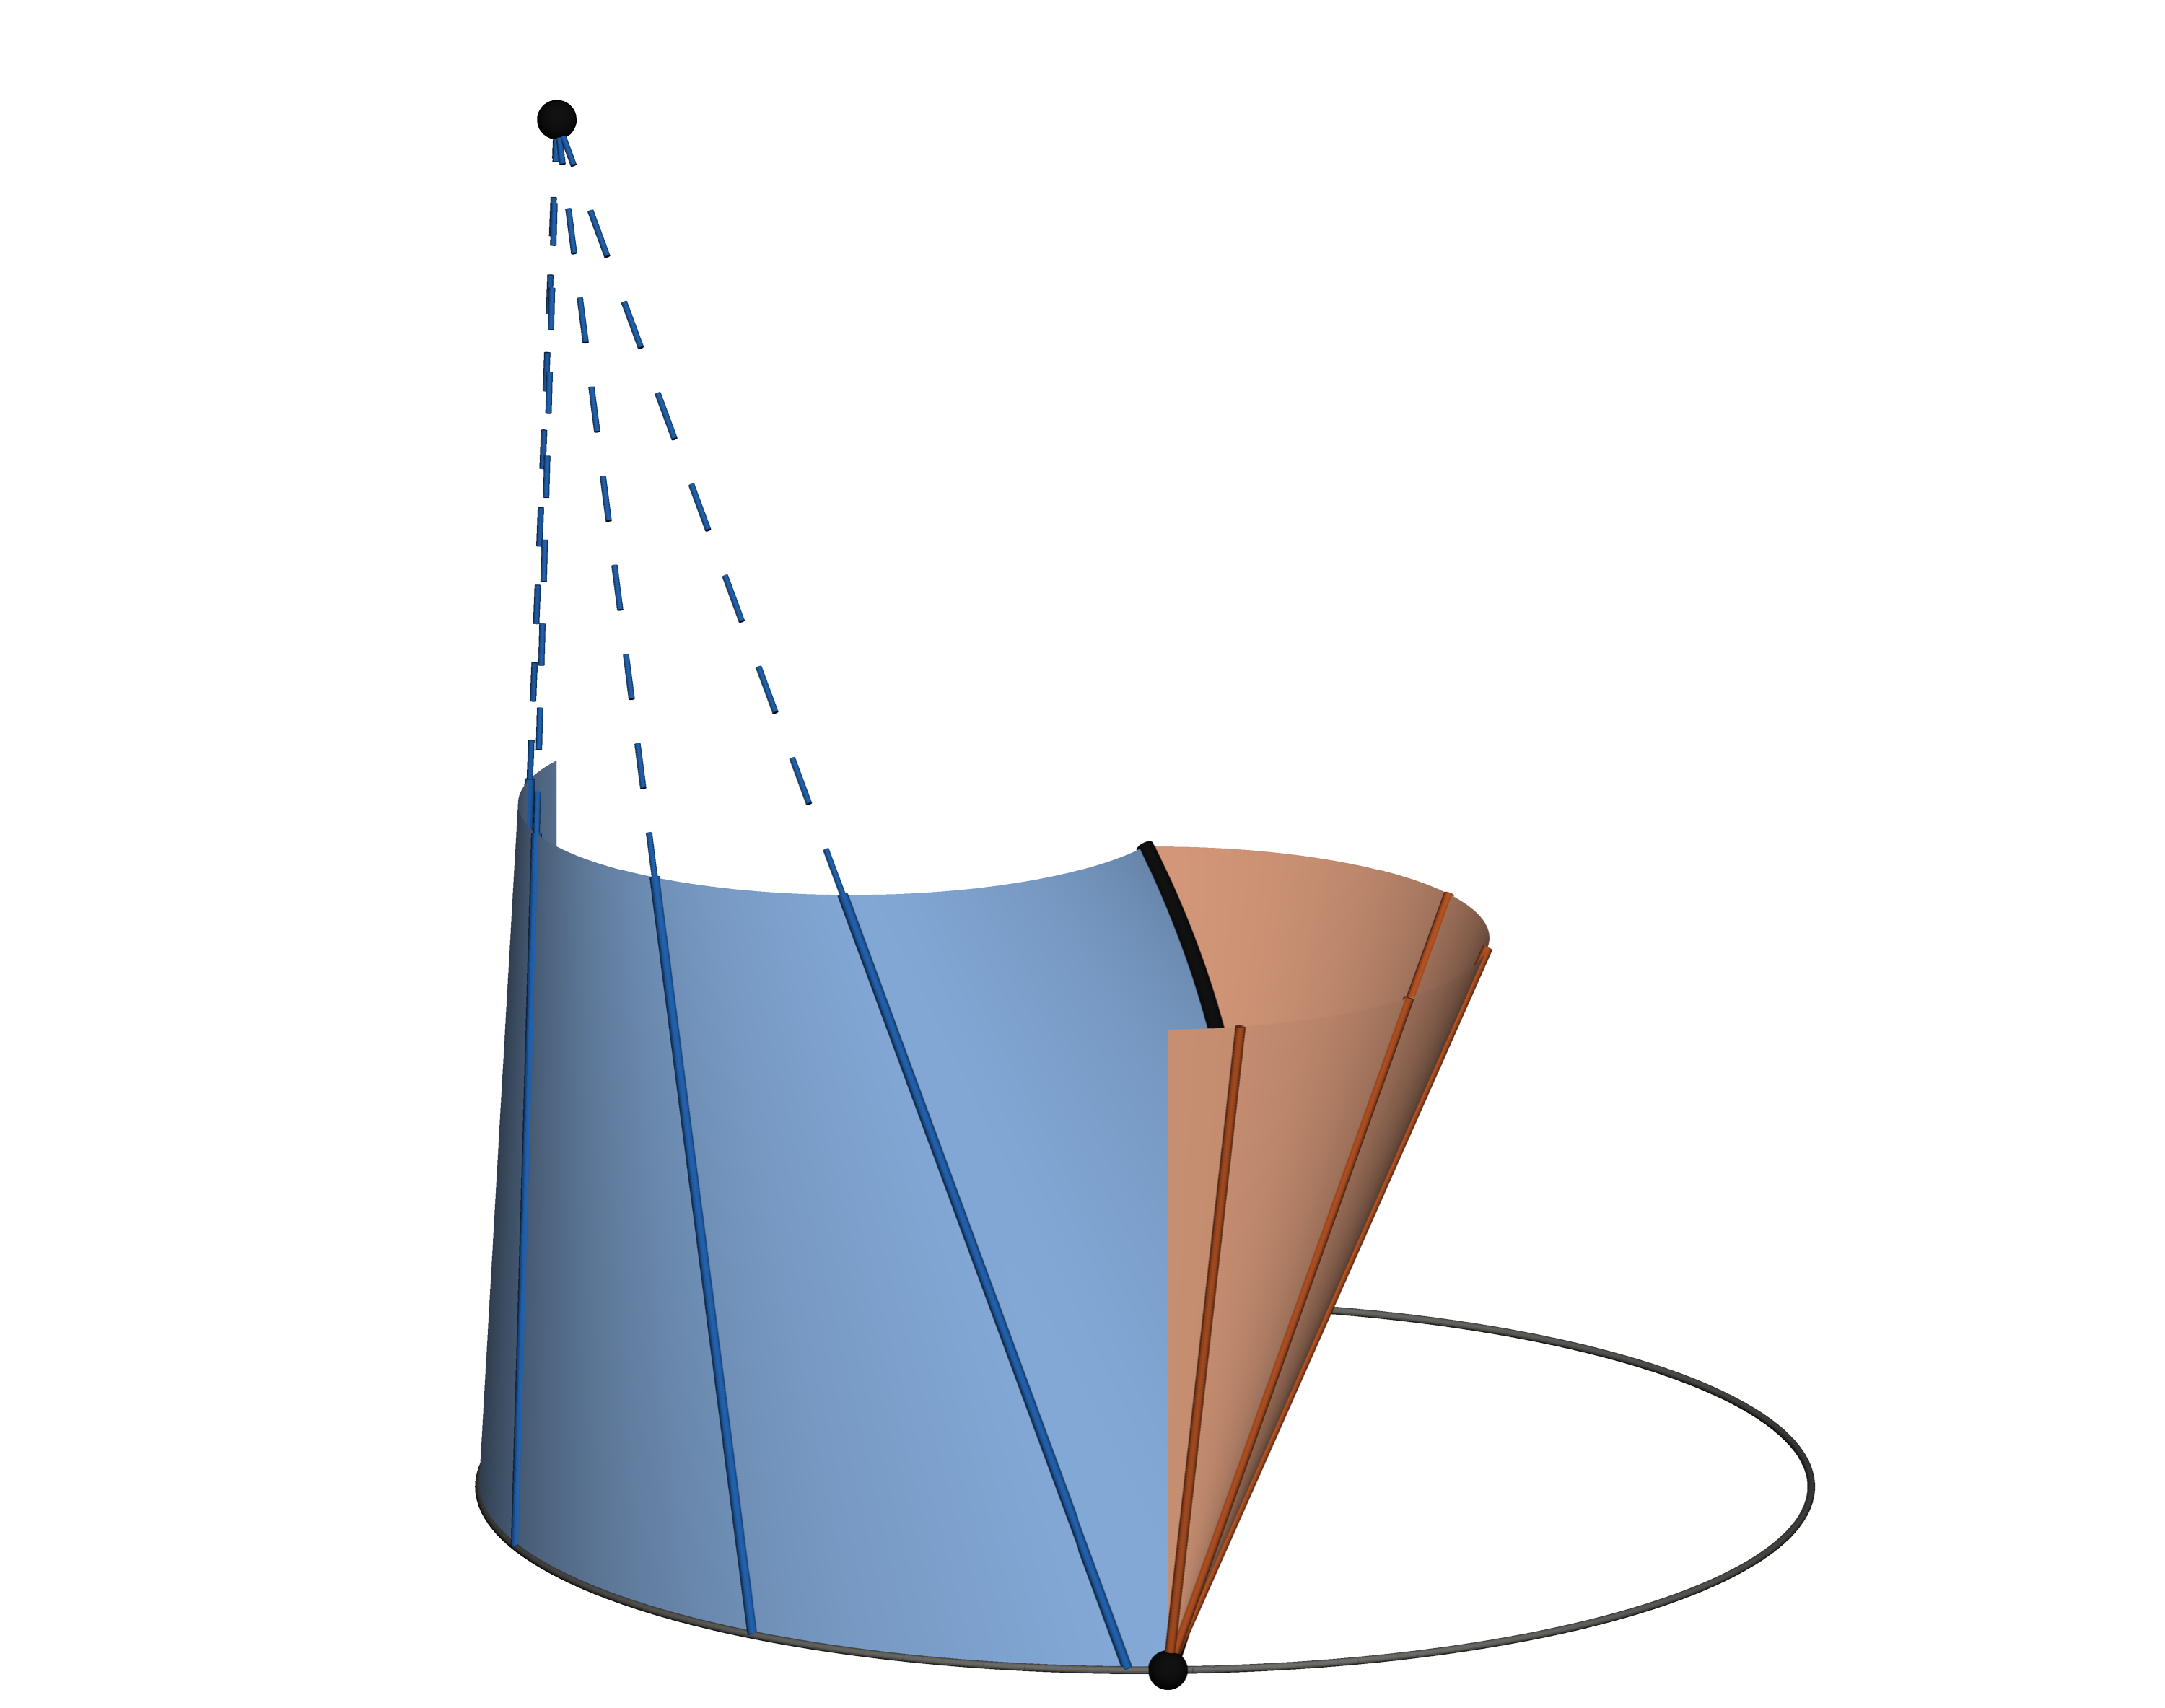
\includegraphics[width=0.43\textwidth]{figures/leaflet3d_a.png}};
\begin{scope}[x={(a.south east)}, y={(a.north west)}]
  \node[lab, anchor=west, xshift=3pt] at (\labAVone) {$V_1=(-1,0,2)$};
  \node[lab, anchor=north west, xshift=2pt] at (\labAVtwo) {$V_2=P$};
  \draw[inktwo, line width=0.4pt] (\labAM) -- ++(0.1,0.13) node[lab, anchor=south west, inner sep=1pt] {$M(z)$};
  \node[lab, anchor=east, xshift=-6pt] at (\labAE) {$E$};
  \node[panel, anchor=north west] at (0,1) {(a)};
\end{scope}
\node[anchor=south west, inner sep=0] (b) at ($(a.south east)+(0.1\textwidth,0)$)
  {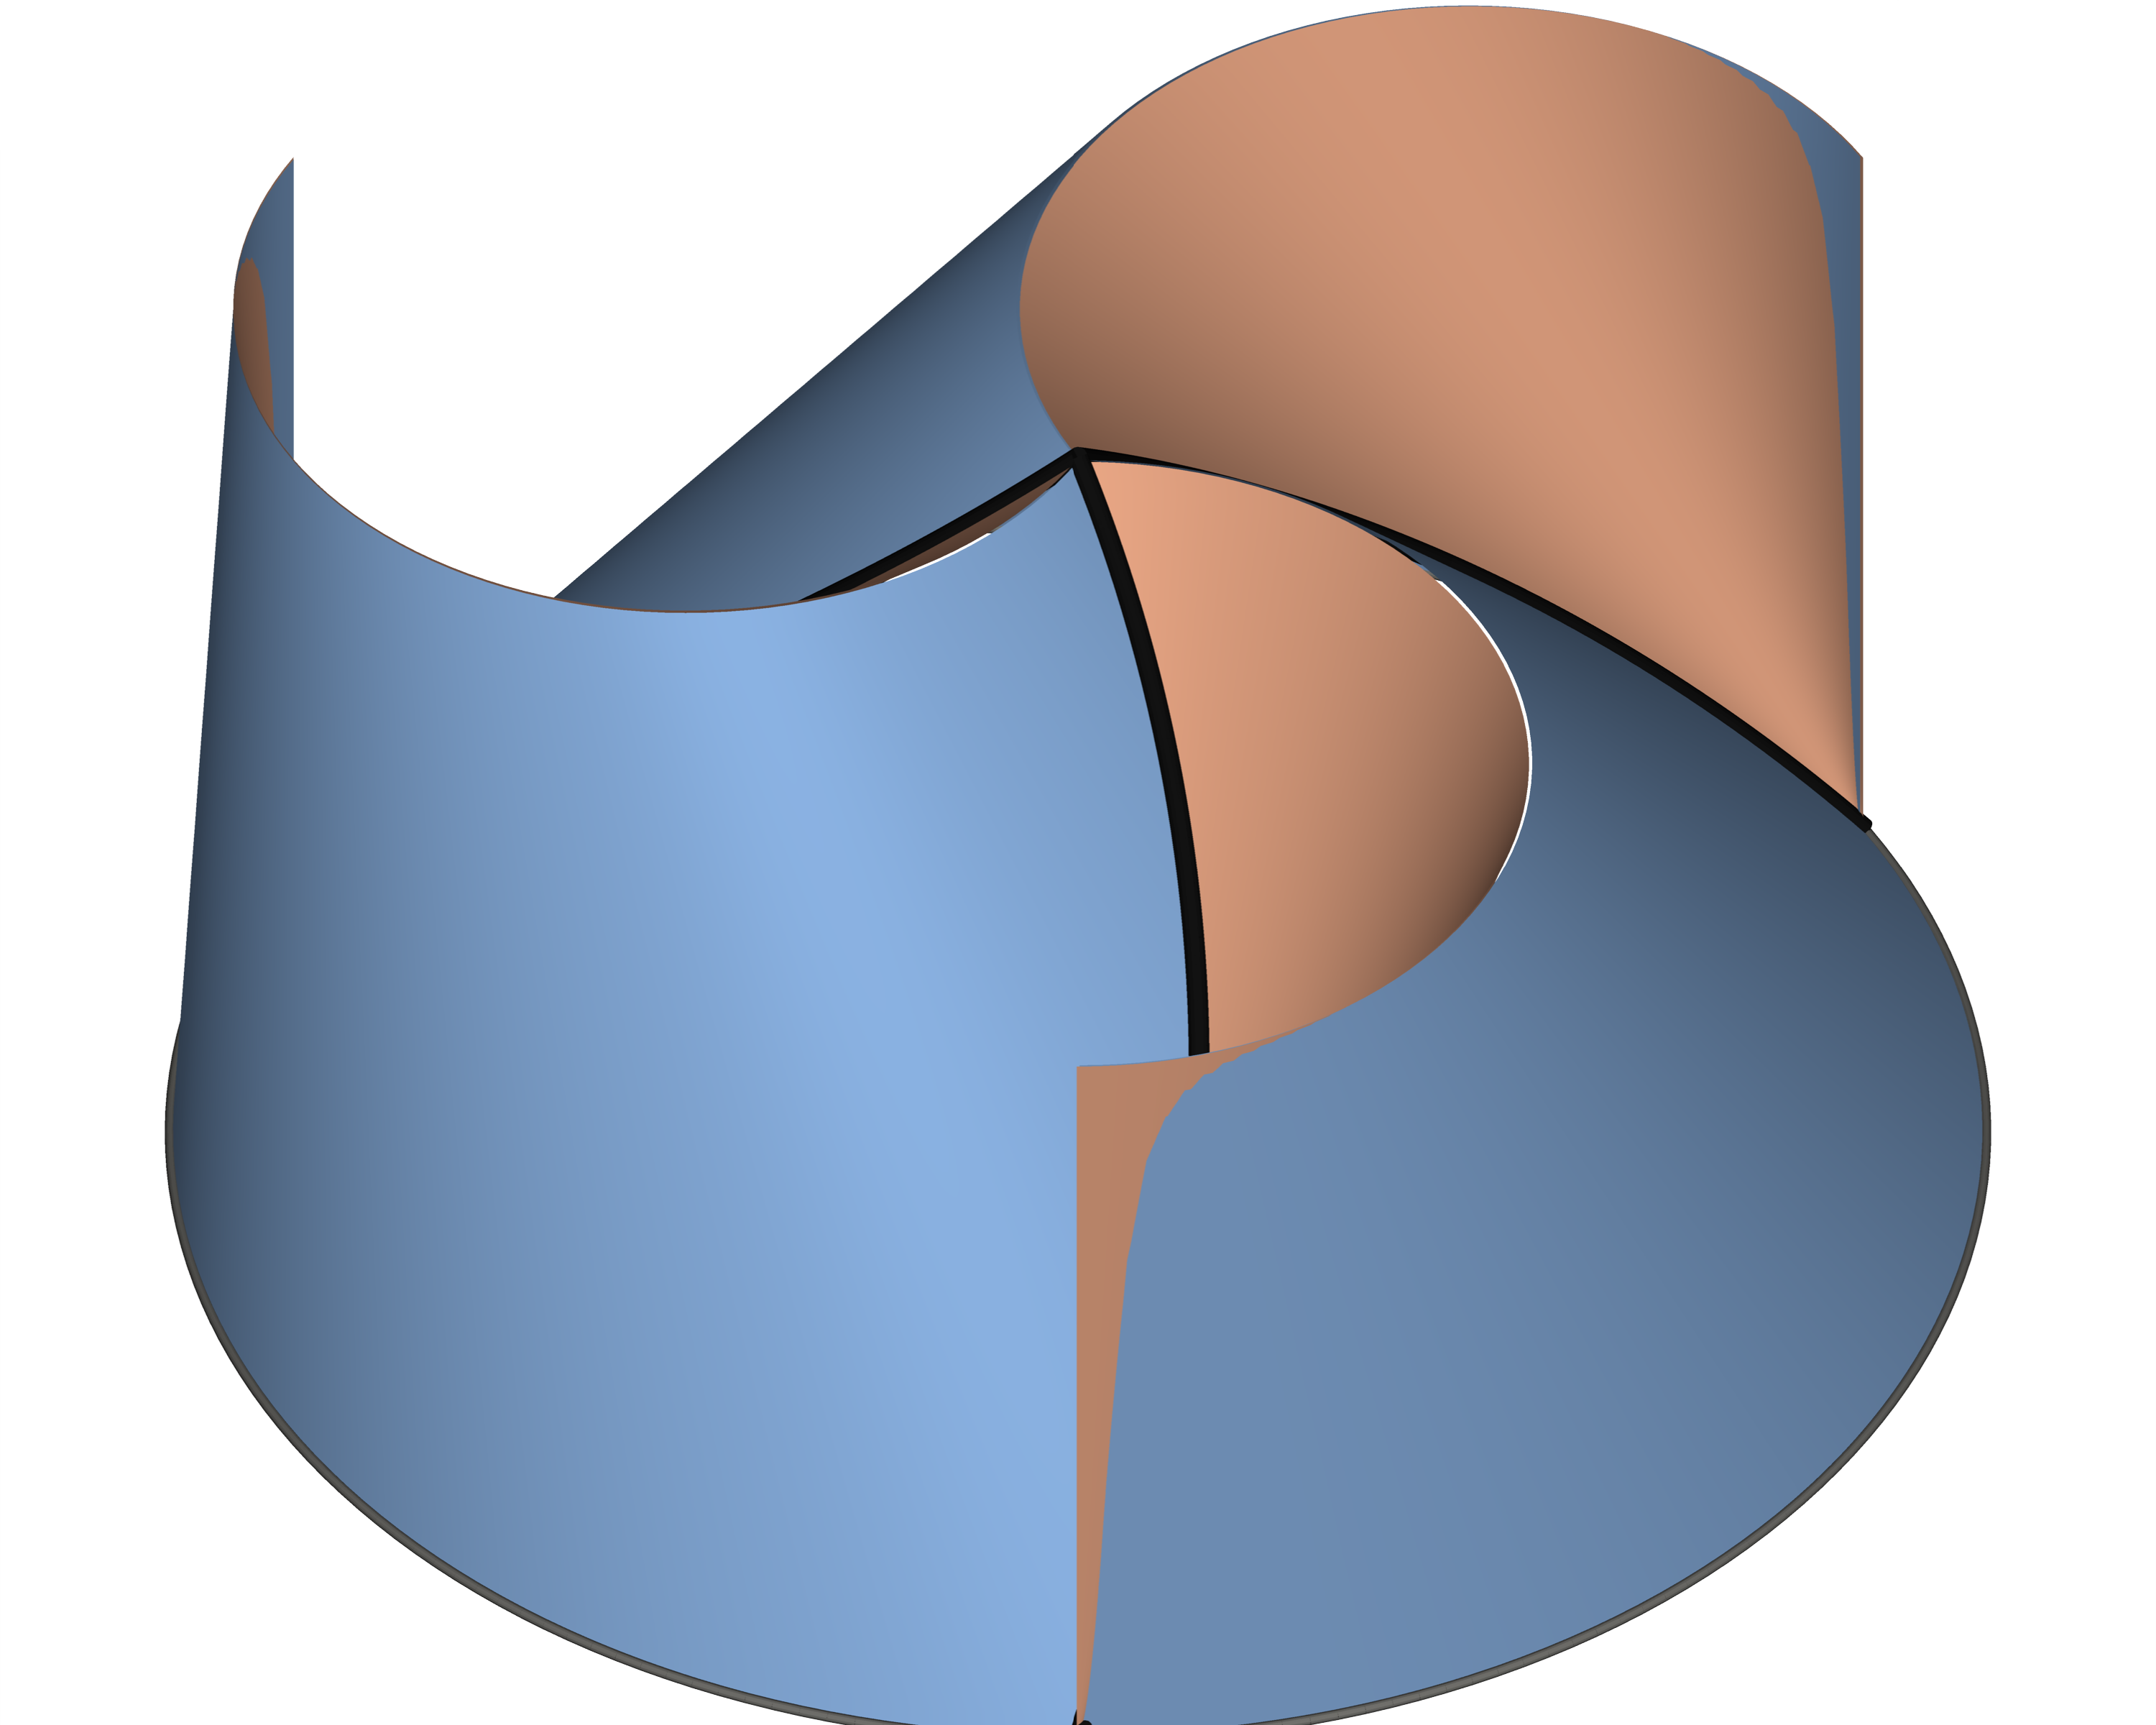
\includegraphics[width=0.43\textwidth]{figures/leaflet3d_b.png}};
\begin{scope}[shift={(b.south west)}, x={($(b.south east)-(b.south west)$)}, y={($(b.north west)-(b.south west)$)}]
  \node[lab, halo, anchor=south, yshift=3pt] at (\labBO) {$O$};
  \node[panel, anchor=north west] at (-0.08,1) {(b)};
\end{scope}
\end{tikzpicture}

\caption{(a) One leaflet ($N=3$). Surface~1 (blue) is a piece of the cone with apex $V_1=(-1,0,2)$, above the valve: its
stays (blue lines) extend (dashed) to $V_1$. Surface~2 (orange) is a piece of the cone with apex $V_2=P$ at the base of the
commissure post, where its stays start. Black: the junction $M(z)$. (b) The three-leaflet valve. Rendered from the exact
parametrisation with an orthographic camera.}
\label{fig:leaflet}
\end{figure}

\begin{theorem}[The whole leaflet is not developable]\label{thm:notflat}\claim{C-011}
Let $k_1,k_2$ be the geodesic curvatures of the junction $M(z)$ as a curve on surface~1 and on surface~2, each measured
with the conormal pointing into its own piece. Then
\[ k_1+k_2=\frac{4\sqrt3\,(z-1)\,\tilde D^2}{\sqrt{\tilde D^2+9}\,(\tilde D^2+12)^{3/2}},\qquad \tilde D=z^2-2z+4, \]
which is negative for $0<z<1$ (value $-5408\sqrt{939}/2146867$ at $z=\tfrac12$) and vanishes at $z=1$. The concentrated
Gaussian curvature carried by the junction is $\int_M(k_1+k_2)\,ds\approx-0.10825$\,rad. Consequently no two-sided
neighbourhood of a point $M(z_0)$, $0<z_0<1$, in the leaflet is intrinsically isometric to a plane region: the leaflet
cannot be obtained from a single flat sheet by bending and folding without stretching.
\end{theorem}
\begin{proof}
The formula for $k_1+k_2$ is a computer-algebra computation from \eqref{eq:X1}--\eqref{eq:X2}, exact at rational heights;
it agrees with the curvatures of the two images of the junction in the flat patterns, computed independently
(\cref{fig:flat}c). An isometry preserves the geodesic curvature of curves \citep[proof of their main
theorem]{FuchsTabachnikov1999}. Suppose that a two-sided neighbourhood of $M(z_0)$, where both pieces and the junction are
regular, were intrinsically isometric to a plane region. Then an arc of $M$ around $M(z_0)$ would be mapped to a single
plane curve with the two pieces on opposite sides of it, so $k_1=-k_2$ along that arc, contradicting $k_1+k_2<0$ on
$(0,1)$. (At $z=1$, $k_1+k_2=0$ at a single point, which proves nothing; $z=0$ is singular.) Equivalently, by Gauss--Bonnet,
two flat pieces glued along a curve form an intrinsically flat surface near that curve only if $k_1+k_2=0$.
\end{proof}

Each half, however, can be cut flat (\cref{thm:flat}). Folding does not help either: a sheet bent and folded without
stretching is still intrinsically flat, and $k_1+k_2=0$ along the crease is the condition that the two sides of a curved
fold of one sheet must satisfy \citep{FuchsTabachnikov1999}, so the leaflet is in particular not a curved fold along $M$.
In the flat patterns, the two images of the junction have equal length ($1.44932$) but different curvature, so they cannot
be sewn edge to edge in the plane. This concerns only manufacture from a flat sheet, the route mentioned by
\citet{Oliveira2024}; moulding or dip-casting are not affected. The Gauss--Bonnet step is classical and not formalised.

\begin{figure}[t]\centering
% Figure: flat patterns of the two halves (true stays, t = const) and the curvature of the two images of the junction.
\begin{tikzpicture}
\begin{axis}[geom, width=0.3\textwidth, name=A]
  \addplot[sone, line width=0.45pt] table {\figdata flat1_z.dat};
  \addplot[sone, line width=0.45pt] table {\figdata flat1_stays.dat};
  \addplot[sone, line width=1.3pt] table {\figdata flat1_base.dat};
  \addplot[sone, line width=1.3pt] table {\figdata flat1_top.dat};
  \addplot[ink, line width=1.8pt] table {\figdata flat1_junction.dat};
  \node[lab, text=sone, anchor=west, xshift=2pt] at \ptflatonebase {$z=0$};
  \node[lab, text=sone, anchor=east, xshift=-2pt] at \ptflatonetop {$z=1$};
  \node[lab, anchor=south east, xshift=-1pt, yshift=1pt] at \ptflatoneJ {$M$};
  \node[panel, anchor=south west] at (rel axis cs:0,1.02) {(a)};
\end{axis}
\begin{axis}[geom, width=0.17\textwidth, at={($(A.east)+(0.05\textwidth,0)$)}, anchor=west, name=B]
  \addplot[stwo, line width=0.45pt] table {\figdata flat2_z.dat};
  \addplot[stwo, line width=0.45pt] table {\figdata flat2_stays.dat};
  \addplot[stwo, line width=1.3pt] table {\figdata flat2_top.dat};
  \addplot[ink, line width=1.8pt] table {\figdata flat2_junction.dat};
  \node[dot] at (axis cs:0,0) {};
  \node[lab, anchor=north east] at (axis cs:0,0) {$V_2$};
  \node[lab, text=stwo, anchor=west, xshift=2pt] at \ptflattwotop {$z=1$};
  \node[lab, anchor=east, xshift=-2pt] at \ptflattwoJ {$M$};
  \node[panel, anchor=south west] at (rel axis cs:0,1.02) {(b)};
\end{axis}
\begin{axis}[graph, width=0.27\textwidth, height=0.24\textwidth, at={($(B.east)+(0.17\textwidth,0)$)}, anchor=west,
             xmin=0, xmax=1, xlabel={$z$},
             legend style={draw=none, fill=none, font=\footnotesize, at={(0.98,0.03)}, anchor=south east},
             legend cell align=left]
  \addplot[sone, name path=kone] table {\figdata kg1.dat};
  \addplot[stwo, name path=ktwo] table {\figdata kg2neg.dat};
  \addplot[faint, forget plot] fill between[of=kone and ktwo];
  \legend{$k_1$, $-k_2$}
  \node[panel, anchor=south west] at (rel axis cs:-0.28,1.02) {(c)};
\end{axis}
\end{tikzpicture}

\caption{Flat patterns of (a) surface~1 and (b) surface~2 (\cref{thm:flat}); thin lines are images of $z=\mathrm{const}$
and of stays ($t=\mathrm{const}$), black is the image of the junction $M$. (c) Geodesic curvature of the junction on each
side, measured towards its own piece, computed from the flat patterns. Sewing the two patterns along $M$ would require
$k_1=-k_2$; the shaded gap is $-(k_1+k_2)>0$ and agrees with the closed form of \cref{thm:notflat} to $10^{-4}$.}
\label{fig:flat}
\end{figure}

%======================================================================
\section{The junction is a crease}\label{sec:crease}

Both pieces lie on the same side $t\le t_M$ of the junction, so a consistent orientation of the leaflet reverses the
normal of one of them. We define the fold angle $\delta$ as the angle between $X_{1,t}\times X_{1,z}$ and
$-(X_{2,t}\times X_{2,z})$: $\delta=0$ means tangent-plane continuity.

\begin{lemma}[Fold angle at a common parameter]\label{lem:foldt}
For every $\theta$ and $0<z<2$, at points of the two surfaces with the same parameter $t$,
\[ \cos\delta=\frac{(1+\cos t)^2-4\cos\theta}{4+(1+\cos t)^2}. \]
\end{lemma}
\begin{proof}
By \cref{lem:conemap}, $X_{1,t}\times X_{1,z}=-\frac12(1-\frac z2)\,c_1$ and $-(X_{2,t}\times X_{2,z})=-\frac12\cdot\frac z2\,c_2$;
both factors are negative for $0<z<2$, so $\delta$ is the angle between $c_1$ and $c_2$. By \cref{lem:leafcones},
$c_1\cdot c_2=-4\,(\cos t,\sin t)\cdot R_\theta(\cos t,\sin t)+(1+\cos t)^2=(1+\cos t)^2-4\cos\theta$ and
$|c_1||c_2|=4+(1+\cos t)^2$.
\end{proof}

\begin{theorem}[Fold angle, $N=3$]\label{thm:fold3}\claim{C-003}
For $0<z\le1$,
\[ \cos\delta(z)=\frac{8D^2+9}{16D^2+9},\qquad D=1-\tfrac z2+\tfrac{z^2}4, \]
so $17/25\le\cos\delta\le3/4$, i.e.\ $41.41^\circ\le\delta\le47.16^\circ$, with the minimum at the free edge. The leaflet
is $C^0$ but not $G^1$ along the whole junction.
\end{theorem}
\begin{proof}
At the junction $1+\cos t_M=1+\frac{1+2b-2b^2}{2D}=\frac{3}{2D}$ and $\cos\theta=-\frac12$, so \cref{lem:foldt} gives
$\cos\delta=\big(\frac{9}{4D^2}+2\big)/\big(\frac{9}{4D^2}+4\big)=\frac{8D^2+9}{16D^2+9}$. The function
$u\mapsto(8u+9)/(16u+9)$ is decreasing, and $D^2\in[\frac9{16},1]$ for $b\in[0,\frac12]$, with $D=\frac34$ at $z=1$;
this gives the bounds. Since $\cos\delta<1$ everywhere, the tangent planes never agree along $M$, while the two pieces do
meet along $M$ (\cref{thm:aplusb}).
\end{proof}

\begin{proposition}[Vertical scale]\label{prop:vscale}\claim{C-021}
With vertical scale $h>0$ (the height multiplied by $h$), along the junction of the $N=3$ leaflet, for $0<z\le1$,
\[ \cos\delta_h=\frac{8h^2D^2+9}{16h^2D^2+9}; \]
for $h=1.5$ it ranges over $[49.17^\circ,53.13^\circ]$ instead of $[41.41^\circ,47.16^\circ]$.
\end{proposition}
\begin{proof}
The stretch replaces $w_1,w_2$ by $(\cos t+1,\sin t,-2h)$ and $R_\theta(\cos t+1,\sin t,2h)$, hence $c_1,c_2$ by
$(-2h\cos t,-2h\sin t,-(1+\cos t))$ and $R_\theta(2h\cos t,2h\sin t,-(1+\cos t))$, and the proof of \cref{lem:foldt} gives
$\cos\delta_h=((1+\cos t)^2-4h^2\cos\theta)/(4h^2+(1+\cos t)^2)$. Insert $1+\cos t_M=3/(2D)$ and $\cos\theta=-\frac12$, and
evaluate the monotone expression at $D=\frac34$ and $D=1$.
\end{proof}

Can the crease be rounded while keeping the leaflet developable, so that it can still be formed from flat material? The
two cones cannot be joined to each other directly (\cref{thm:nocommon} and the remark after it); for a rounding through a
strip we only have a local lemma and an expectation, stated below.

\begin{theorem}[No common tangent plane]\label{thm:nocommon}\claim{C-017}
For $N\ge3$ the two cones have no common tangent plane: there are no stays $t_1,t_2$ whose tangent planes coincide. For
$N=2$ the stays $t_1=t_2=2\pi$, which form the junction, do share their tangent plane.
\end{theorem}
\begin{proof}
By \cref{lem:conemap} the tangent plane of cone $i$ along the stay $t$ is the plane through $V_i$ with normal $c_i(t)$
(the whole stay lies in it). The planes for $t_1$ and $t_2$ coincide if and only if $c_1(t_1)\parallel c_2(t_2)$ and
$(V_2-V_1)\cdot c_1(t_1)=0$. A computation gives $(V_2-V_1)\cdot c_1(t_1)=2\,(1+\cos(t_1-\theta))$, so
$t_1\equiv\theta+\pi$ and $c_1(t_1)=(2\cos\theta,\,2\sin\theta,\,-(1-\cos\theta))$. The horizontal parts of $c_1(t_1)$ and
$c_2(t_2)$ both have length $2$, so parallel means $c_2(t_2)=\pm c_1(t_1)$. With the sign $+$, the horizontal parts give
$t_2\equiv0$ and the vertical ones $-2=-(1-\cos\theta)$, i.e.\ $\cos\theta=-1$; with the sign $-$, $t_2\equiv\pi$ and
$0=1-\cos\theta$, i.e.\ $\cos\theta=1$. Neither holds for $N\ge3$. For $N=2$, $\theta=\pi$ and $t_1=t_2\equiv0$ satisfy both
conditions.
\end{proof}

A cone has the same tangent plane along a whole stay. At a point where a piece of cone~1 meets a piece of cone~2 with
tangent-plane continuity, the common tangent plane would be tangent to cone~1 along a stay and to cone~2 along a stay.
Hence, for $N\ge3$, \emph{no} $G^1$ junction between the two cones exists, along any curve.

\begin{lemma}[Local rigidity; classical]\label{lem:rigid}\claim{C-018}
Let $S$ be a regular surface of class $C^\infty$ with $K\equiv0$. Suppose $S$ contains an open piece $C_0$ of a cone, away
from its apex, such that the second fundamental form $\mathrm{II}$ of the cone never vanishes on $C_0\cup\gamma$, and let
$\gamma\subset S$ be a curve in the interior of $S$ that bounds $C_0$ and is transversal to the stays. Then near every
interior point of $\gamma$, $S$ coincides with that cone.
\end{lemma}
The hypothesis $\mathrm{II}\ne0$ cannot be dropped: a non-planar cone may contain planar regions, and a developable surface
can leave the cone through one of them.\footnote{The graph of $y\,\varphi(x/y-1)$ with $\varphi(s)=e^{-1/s^2}$ for $s>0$,
$\varphi(s)=0$ for $s\le0$ is a non-planar cone that is planar where $x<y$; on $|x|<1/4$ it is planar for $1/2<y<1$ and is
continued for $1\le y<3/2$ by the graph of $\varphi(y-1)$.} For the two cones of the leaflet it holds at every regular
point: $X_{tt}=(\alpha+\beta z)w''$, so the $tt$ coefficient of $\mathrm{II}$ is a non-zero multiple of
$w''\cdot(w'\times w)$, which equals $2$ for $w_1$ and $-2$ for $w_2$; the other two coefficients vanish
(\cref{lem:conemap}). So $\mathrm{II}\ne0$ for $z\ne2$ on surface~1 and $z\ne0$ on surface~2.
\begin{proof}
We use two classical facts for smooth surfaces with $K\equiv0$ \citep[\S5-8, Propositions~1 and~2, due to
Massey]{doCarmo1976}: through a parabolic point (where $K=0$ and $\mathrm{II}\ne0$) there passes a unique asymptotic line,
which is an open segment of a straight line along which the unit normal, hence the tangent plane, is constant; and a
maximal such segment never meets a planar point. Since $S$ is smooth and coincides with the cone on $C_0$, its second
fundamental form at a point $q\in\gamma$ is, by continuity from $C_0$, that of the cone at $q$, which is non-zero by
hypothesis (for the leaflet's cones, $q$ lies on a stay that enters $C_0$ by transversality, away from the apex, where
$L\ne0$); by continuity every point of $S$ near $q$ is parabolic and the asymptotic direction field is continuous there.
The asymptotic line of $S$ through a point of $C_0$ is the stay of the cone through it (uniqueness), so the stays are
straight segments of $S$ that cross $\gamma$. Let $r\in S$ be close to $q$ on the other side of $\gamma$. Its asymptotic
segment is straight, with direction close to that of the stay through $q$, and extends until it leaves a fixed
neighbourhood of $q$ in the interior of $S$ (it cannot end at a planar point). Since $\gamma$ is transversal to the stays,
the segment crosses $\gamma$ at a point $q'$ near $q$, where it must coincide with the stay through $q'$. Hence $r$ lies
on the extension of a stay, that is, on the cone.
\end{proof}
The smoothness assumption comes from the reference. Versions for lower regularity exist \citep[e.g.][]{HartmanNirenberg1959},
but we have not checked their exact hypotheses.

\begin{remark}[Expected, not proved]\label{rem:expected}
We expect that for $N\ge3$ no $C^\infty$ developable surface agrees with the leaflet outside a thin strip around the
junction $M$ (restricted to heights $z$ in a compact subinterval of $(0,1)$). By \cref{lem:rigid}, the stays of both cones
would continue as straight lines into the strip, and where a continued stay of one cone reaches the other piece the two
tangent planes would have to agree, which \cref{thm:nocommon} excludes. Making this precise requires controlling where the
continued stays leave the strip; we have not done this.
\end{remark}

\paragraph{A $G^1$ rounding.}\claim{C-019} In each horizontal section $0<z\le1$, replace a neighbourhood of $M$ by the
circular arc of radius $\rho(z)=\rho_0 z$ tangent to both section circles. Each section is then $G^1$ and the family varies
smoothly with $z$, so the surface is $G^1$. The rounded strip is not developable: numerically $K$ reaches about $-38$
(normalised units, $\rho_0=0.05$), and for $\rho_0=0.1$ it is non-zero at every sample with $\max|K|>1$. This is consistent
with \cref{rem:expected}. The mechanical comparison of \cref{sec:fem} uses a variant with radius $\sqrt{(\rho_0z)^2+(T/R)^2}$
(never thinner than the shell), which is smooth in $z$, and removes the corner at the base of the commissure post where the
rounding cannot be thickened. For $N=2$ the junction is a common stay with a common tangent plane (\cref{thm:foldN}), and no
rounding is needed. \citet{Oliveira2024} report bending of the leaflets near the centre in diastole for the 2021 geometry;
whether a crease of this kind plays a role there is not addressed in this note.

%======================================================================
\section{$N$ leaflets}\label{sec:N}

\begin{theorem}[The relation $a=1-b$ does not depend on $N$]\label{thm:aplusb}\claim{C-012}
Let $\cos\theta\ne1$. If the large circle $\{(a-1+a\cos t,\ a\sin t)\}$ and the small circle
$\{(b-1+b\cos t,\ b\sin t)\}$ rotated by $\theta$ share a point with the same parameter $t$ on both, then $a+b=1$. Assume
further $0<\theta\le\pi$ (true for $\theta=2\pi/N$), $0\le b\le\frac12$ and $a=1-b$. Then the two surfaces meet at the same parameter
\[ t_M^\theta=2\pi-\arccos\frac{2ab-(a^2+b^2)\cos\theta}{\Delta},\qquad \Delta=a^2+b^2-2ab\cos\theta>0, \]
which equals $t_M$ for $N=3$. The junction runs from $t_M^\theta=\pi+\theta$, $M=R_\theta E$, at $z=0$ to $t_M^\theta=2\pi$, $M=O$, at $z=1$.
\end{theorem}
\begin{proof}
Write $e=(1,0)$, $u=(\cos t,\sin t)$ and $v=e+u$. The two points are $p=av-e$ and $q=bv-e$, and $p=R_\theta q$, so
$|p|=|q|$. Since $|sv-e|^2=1-s(1-s)|v|^2$, this gives $(a-b)(1-a-b)|v|^2=0$. If $v=0$ then $p=q=-e$ and $-e=R_\theta(-e)$
forces $\cos\theta=1$, which is excluded. If $a=b$ then $p=q=R_\theta p$, so $p=0$, i.e.\ $av=e$; hence $\sin t=0$,
$\cos t=1$, $v=2e$ and $a=b=\frac12$. In every remaining case $a+b=1$.

For the junction, note first that $\Delta=(a-b)^2+2ab(1-\cos\theta)>0$ for $b\in[0,\frac12]$, $a=1-b$ and
$\cos\theta<1$ (if $b=0$ then $\Delta=1$). Let $c=(2ab-(a^2+b^2)\cos\theta)/\Delta$ and $s=(b^2-a^2)\sin\theta/\Delta$. With $a=1-b$ one checks
$c^2+s^2=1$ and that \eqref{eq:X1} and \eqref{eq:X2} coincide at $(\cos t,\sin t)=(c,s)$. For $0<\theta\le\pi$ and
$b\le\frac12$, $s\le0$, so $t=2\pi-\arccos c\in[\pi,2\pi]$. At $z=0$ ($a=1$, $b=0$), $(c,s)=(-\cos\theta,-\sin\theta)$, so
$t=\pi+\theta$ and $M=(\cos(\pi+\theta),\sin(\pi+\theta))=R_\theta E$; at $z=1$ ($a=b=\frac12$), $(c,s)=(1,0)$, so $t=2\pi$ and
$M=O$. For $\theta=2\pi/3$, $c=(1+2b-2b^2)/(2D)$, the paper's value.
\end{proof}

\begin{theorem}[Fold angle for $N$ leaflets]\label{thm:foldN}\claim{C-014}
For $0<z\le1$, along the junction, with $X=1+\cos t_M^\theta=(1-\cos\theta)/\Delta$,
\[ \cos\delta=\frac{X^2-4\cos\theta}{X^2+4}. \]
Hence the junction is a crease if and only if $\cos\theta\ne-1$, i.e.\ for every $N\ge3$. For $N=2$ the junction is the
common stay $t=2\pi$ and the leaflet is $G^1$. At the free edge $\cos\delta=\sin^2(\pi/N)$.
\end{theorem}
\begin{proof}
With $a+b=1$, $1+c=\big((a^2+b^2)(1-\cos\theta)+2ab(1-\cos\theta)\big)/\Delta=(1-\cos\theta)/\Delta$; insert this in
\cref{lem:foldt}. Then $\cos\delta<1$ if and only if $\cos\theta>-1$. For $\theta=\pi$, $c=1$ for every $z$, so
$t_M\equiv2\pi$ and $\cos\delta=1$. At $z=1$, $\Delta=\frac12(1-\cos\theta)$ and $X=2$, so
$\cos\delta=(1-\cos\theta)/2=\sin^2(\theta/2)$.
\end{proof}

\begin{figure}[t]\centering
% Figure: fold angle along the junction, N = 2..7 (h = 1), and N = 3 with h = 1.5.
\begin{tikzpicture}
\begin{axis}[graph, width=0.55\textwidth, height=0.42\textwidth, xmin=0, xmax=1, ymin=-6, ymax=132,
             ytick={0,30,60,90,120}, xlabel={$z$}, ylabel={$\delta$ ($^\circ$)}]
  \addplot[rtwo] table {\figdata fold2.dat} node[pos=0.02, anchor=south west, inner sep=1pt, font=\footnotesize, text=muted] {$N=2$};
  \addplot[rthree, line width=1.4pt] table {\figdata fold3.dat} node[pos=0.55, anchor=north, inner sep=2pt, font=\footnotesize, text=rthree] {$N=3$};
  \addplot[rfour] table {\figdata fold4.dat} node[pos=0.02, anchor=south west, inner sep=1pt, font=\footnotesize, text=rfour] {$N=4$};
  \addplot[rfive] table {\figdata fold5.dat} node[pos=0.02, anchor=south west, inner sep=1pt, font=\footnotesize, text=rfive] {$N=5$};
  \addplot[rsix] table {\figdata fold6.dat} node[pos=0.02, anchor=south west, inner sep=1pt, font=\footnotesize, text=rsix] {$N=6$};
  \addplot[rseven] table {\figdata fold7.dat} node[pos=0.02, anchor=south west, inner sep=1pt, font=\footnotesize, text=rseven] {$N=7$};
  \addplot[rthree, dashed] table {\figdata fold3_h15.dat}
    node[pos=0.55, anchor=south, font=\footnotesize, text=rthree, yshift=1pt] {$N=3,\ h=\pgfmathprintnumber{1.5}$};
\end{axis}
\end{tikzpicture}

\caption{Fold angle $\delta$ along the junction for $N=2,\dots,7$ (vertical scale $h=1$, \cref{thm:foldN}) and for $N=3$
with $h=1.5$ (dashed, \cref{prop:vscale}). For $N\ge5$ the fold exceeds $90^\circ$ near the base; for $N=2$ there is no crease.}
\label{fig:fold}
\end{figure}

\begin{theorem}[The free edges close for every $N$]\label{thm:freeedge}\claim{C-013}
At $z=1$, $X_2(t,1)=R_\theta X_1(t,1)$ for all $t$: the second piece of leaflet $k$ coincides pointwise with the first piece
of leaflet $k+1$. The free edges are $N$ semicircles of radius $\frac12$ joining the centre to the commissures
(\cref{fig:top}).
\end{theorem}
\begin{proof}
At $z=1$, $a=b=\frac12$, so both \eqref{eq:X1} and the argument of $R_\theta$ in \eqref{eq:X2} equal
$(-\frac12+\frac12\cos t,\ \frac12\sin t,\ 1)$, the circle of radius $\frac12$ centred at $(-\frac12,0,1)$; $t\in[\pi,2\pi]$
runs over the half from $E$ to $O$.
\end{proof}

The cone congruence $T(X_1(t,z))=X_2(t,2-z)$ of \cref{prop:congruent} holds for every $\theta$ with the same proof. At $z=1$
all free edges meet at the centre, so for $N\ge4$ non-neighbouring leaflets touch there. Below the free edge, at the 25
sampled heights $z\in[0.02,0.98]$, non-neighbouring leaflets do not touch ($N=2,\dots,7$).

\begin{figure}[t]\centering
% Figure: top views of the N-leaflet valves; thin: sections z = 1/4, 1/2, 3/4; thick: free edges (z = 1).
\newcommand{\topview}[1]{%
  \addplot[muted, dashed, line width=0.45pt] table {\figdata ring.dat};
  \addplot[sone, line width=0.5pt, opacity=0.6] table {\figdata top#1_sec1.dat};
  \addplot[stwo, line width=0.5pt, opacity=0.6] table {\figdata top#1_sec2.dat};
  \addplot[sone, line width=1.5pt] table {\figdata top#1_edge1.dat};
  \addplot[stwo, line width=1.5pt] table {\figdata top#1_edge2.dat};}
\begin{tikzpicture}
\begin{groupplot}[group style={group size=4 by 1, horizontal sep=0.035\textwidth}, geom, width=0.21\textwidth,
                  xmin=-1.05, xmax=1.05, ymin=-1.05, ymax=1.05, title style={font=\small, yshift=-3pt}]
  \nextgroupplot[title={$N=2$}] \topview{2}
  \nextgroupplot[title={$N=3$}] \topview{3}
  \nextgroupplot[title={$N=4$}] \topview{4}
  \nextgroupplot[title={$N=6$}] \topview{6}
\end{groupplot}
\end{tikzpicture}

\caption{Top views of the $N$-leaflet valves: sections at $z=\frac14,\frac12,\frac34$ (thin) and free edges $z=1$ (thick),
which close for every $N$ (\cref{thm:freeedge}). Surface~1 blue, surface~2 orange.}
\label{fig:top}
\end{figure}

%======================================================================
\section{Area and coaptation}\label{sec:area}

\begin{proposition}[Area]\label{prop:area}\claim{C-015}
For $0\le z\le2$, $|X_{1,t}\times X_{1,z}|+|X_{2,t}\times X_{2,z}|=\tfrac12\sqrt{4+(1+\cos t)^2}$, independently of $z$ and
$N$. Hence the area of one leaflet is
\[ A_N=\frac12\int_0^1\!\!\int_\pi^{t^\theta_M(z)}\sqrt{4+(1+\cos t)^2}\,dt\,dz, \]
with $A_3\approx2.89364$ (radius 1, $h=1$). Numerically, the total area $N A_N$ increases with $N$ for every tested value
$N=2,\dots,30$: $7.305$, $8.681$, $9.889$, $10.938$, $11.856$, $12.668$ for $N=2,\dots,7$, and $21.237$ for $N=30$. We have no
proof for every $N$.
\end{proposition}
\begin{proof}
By \cref{lem:conemap,lem:leafcones}, $|X_{1,t}\times X_{1,z}|=\frac12(1-\frac z2)|c_1|$ and
$|X_{2,t}\times X_{2,z}|=\frac12\cdot\frac z2|c_2|$, and $|c_1|=|c_2|=\sqrt{4+(1+\cos t)^2}$; the coefficients add up to
$\frac12$ for $0\le z\le2$. Both pieces are parametrised over the same $\Omega$. The values are quadratures.
\end{proof}

So in this natural $N$-family the total leaflet area is \emph{not} preserved. The family $G_N(\alpha)$ of the talk is not
defined precisely enough for us to test the claim made there.

\begin{proposition}[Coaptation]\label{prop:coapt}\claim{C-016}
Let $0\le z<1$. For each pair of facing pieces, piece~2 of leaflet $k$ and piece~1 of leaflet $k+1$, the sections lie on two
circles internally tangent at their common commissure, so they meet only there; at $z=1$ they coincide along the whole free
edge. (For $N=2$ the two leaflets face each other across both commissures.) The geometric orifice area of the unloaded
design is zero.
\end{proposition}
\begin{proof}
Piece~2 of leaflet $k$ is $R_\theta$ of the circle with centre $(-a,0)$ and radius $b$, and piece~1 of leaflet $k+1$ is
$R_\theta$ of the circle with centre $(-b,0)$ and radius $a$. Both circles pass through $E$ and their centres are $a-b$ apart,
the difference of the radii; for $a\ne b$ ($z<1$) they are internally tangent at $E$ and have no other common point. At
$z=1$ use \cref{thm:freeedge}. The projections cover the disk without gaps (\cref{prop:cover}), so the unloaded orifice area
is zero.
\end{proof}
The other pairs of pieces were only sampled. For $N=2,\dots,7$ we took 4000 parameter values per section at 25 equally
spaced heights $z\in[0.02,0.98]$, discarding points within distance $0.02$ of any commissure post ($R=1$); the minimum distance
between retained sample points of non-facing pieces of neighbouring leaflets was about $0.0121$. Together with the sampled
check of non-neighbouring leaflets (\cref{sec:N}), these observations are consistent with zero free coaptation area and height,
excluding the attachment posts. They do not establish the absence of contacts between the samples or in the excluded
regions.

%======================================================================
\section{Comparing different numbers of leaflets}\label{sec:compare}

A study that compares $N=2,3,4,\dots$ needs a rule saying what is kept fixed. We keep the \emph{total leaflet area} fixed
and treat the opening area as a response. Here $R$ is the ring radius and $H$ the height; the section at height $Hs$ uses
the parameter $z=g(s)$, where the vertical profile $g$ belongs to
$\mathcal G=\{g\in C^1([0,1]):\ g'\ge0,\ g(0)=0,\ g(1)=1\}$ (the paper uses $g(s)=s$).

\begin{proposition}[Area density and scaling]\label{prop:scaling}\claim{C-024}\claim{C-031}
For $0\le g\le 2$, $|X_{1,t}\times X_{1,s}|+|X_{2,t}\times X_{2,s}|=\tfrac R2\sqrt{4H^2+R^2g'(s)^2(1+\cos t)^2}$; for
$0\le g\le1$ the two pieces form the leaflet, and we use only that range (for $N\ge3$ and larger $g$ the pieces no longer
meet along the junction; for $N=2$ they still do). Hence the total area of the $N$ leaflets is
$R^2 A^{\mathrm{tot}}_N(H/R,g)$, with $A^{\mathrm{tot}}_N=N A_N$ in the notation of \cref{prop:area}: every dimensionless
quantity (fold angle, opening area$/\pi R^2$) depends only on $N$, $g$ and $h=H/R$. Fixing the area together with $R$, or
together with $H$, selects \emph{different} shapes of this family, not the same shape at two scales.
\end{proposition}
\begin{proof}
A direct computation gives $|X_{1,t}\times X_{1,s}|=\frac R2(1-\frac g2)\sqrt{4H^2+R^2g'^2(1+\cos t)^2}$ and
$|X_{2,t}\times X_{2,s}|=\frac R2\cdot\frac g2\sqrt{4H^2+R^2g'^2(1+\cos t)^2}$. Integrating over
$\{0\le s\le1,\ \pi\le t\le t_M(g(s))\}$ and writing $H=hR$ factors out $R^2$.
\end{proof}

\begin{proposition}[Projected area and covering]\label{prop:cover}\claim{C-027}
For every integer $N\ge2$, $R,H>0$ and every $g\in\mathcal G$, the top-view projections of the $N$ leaflets cover the disk
of radius $R$ with multiplicity one almost everywhere; in particular their areas add up to $\pi R^2$ and the unloaded
design has zero geometric orifice area.
\end{proposition}
\begin{proof}
Orient piece~1 by $(t,z)$ and piece~2 oppositely; the projected Jacobians are then $R^2a(1+\cos t)/2\ge0$ and
$R^2b(1+\cos t)/2\ge0$. For a test function $f$ on the plane, write $f\,dx\wedge dy=d\alpha$ and apply Stokes to each piece.
Summing over pieces and leaflets, the junctions cancel (same curve, opposite orientations), the free edges cancel between
neighbouring leaflets (\cref{thm:freeedge}), the posts and the base of piece~2 project to points, and the bases of the
pieces~1 make up the circle of radius $R$ once, counter-clockwise. Hence $\sum\int f(F)\,|J|=\int_{\text{disk}}f$, so by the
area formula the multiplicity of the projection is $1$ almost everywhere on the disk and $0$ outside; since the union of the
images is compact, no point of the open disk is missed. The profile $g$ only reparametrises the heights and does not
change the argument.
\end{proof}

\subsection{Keeping $R$ and $H$ fixed}
With the paper's linear profile the total area grows with $N$ (\cref{prop:area}), so a fair comparison must change
something. If $R$ and $H$ are both kept, only the profile $g\in\mathcal G$ is free, and the geometry limits what it can do.
We take $R=1$.

\begin{proposition}[Two leaflets]\label{prop:two}\claim{C-025}\claim{C-028}
For $N=2$ and every $H>0$, the linear profile has the least total area in $\mathcal G$, uniquely, and every value in
$[A^{\mathrm{tot}}_2(H,s),\ \pi(2H+1))$ is the total area of some $g\in\mathcal G$.
\end{proposition}
\begin{proof}
For $\theta=\pi$, $t_M\equiv2\pi$ (\cref{thm:foldN}), so the total area is $\int_\pi^{2\pi}\!\int_0^1\phi_t(g'(s))\,ds\,dt$ with
$\phi_t(p)=\sqrt{4H^2+p^2(1+\cos t)^2}$, strictly convex in $p$ for $t\ne\pi$. As $\int_0^1g'=1$, Jensen's inequality gives
$\int_0^1\phi_t(g')\ge\phi_t(1)$, with equality only for $g'\equiv1$. Also $\phi_t(p)\le2H+p(1+\cos t)$, with strict inequality when $p>0$ and $t>\pi$; since $g'$ is continuous with
$\int_0^1g'=1$, it is positive on a set of positive measure, so the total area is strictly below $\pi(2H+1)$. Profiles whose
derivative concentrates near one height approach this value. Finally $\mathcal G$ is convex and
the area is continuous on it (in the $C^1$ topology), so along segments of $\mathcal G$ every intermediate value is attained.
\end{proof}

Reaching the area of the linear $N=3$ design with $N=2$ at $H=R$ takes very steep profiles in the families we tried
($s^m$ with $m\approx17$).

\begin{proposition}[A lower bound over all profiles]\label{prop:lower}\claim{C-029}
For $N\ge3$, $\theta=2\pi/N$, $c(t)=1+\cos t$ and $\mu(t)=|\{z\in[0,1]: t_M^\theta(z)\ge t\}|$, every $g\in\mathcal G$ satisfies
\[ A^{\mathrm{tot}}_N(H,g)\ \ge\ LB_N(H)=\frac N2\Big[\int_\pi^{\pi+\theta}\!\sqrt{4H^2+c^2}\,dt+\int_{\pi+\theta}^{2\pi}c(t)\,\mu(t)\,dt\Big]. \]
At $H=1$, $LB_N$ exceeds the total area $8.6809$ of the linear $N=3$ design for $N=5,6,7$ (quadrature, error below $10^{-13}$),
so no profile gives those $N$ that area.
\end{proposition}
\begin{proof}
For any measurable $\varphi(t)\in[0,\pi/2]$ and $p,c\ge0$, $\sqrt{4H^2+p^2c^2}\ge2H\cos\varphi+pc\sin\varphi$ (Cauchy--Schwarz).
Take $\tan\varphi=c/(2H)$ on $[\pi,\pi+\theta]$ and $\varphi=\pi/2$ on $(\pi+\theta,2\pi]$. Since $t_M(g(s))\ge\pi+\theta$ for
every $s$, the $2H\cos\varphi$ part integrates over $[\pi,\pi+\theta]$ only. For the other part, the substitution $z=g(s)$ and
Fubini give $\int_0^1g'(s)\int_\pi^{t_M(g(s))}c\sin\varphi\,dt\,ds=\int_\pi^{2\pi}c(t)\sin\varphi(t)\,\mu(t)\,dt$. On
$[\pi,\pi+\theta]$, $\mu=1$ and $2H\cos\varphi+c\sin\varphi=\sqrt{4H^2+c^2}$ at the chosen $\varphi$.
\end{proof}

\begin{proposition}[Four leaflets]\label{prop:four}\claim{C-030}
At $H=R$, every $g\in\mathcal G$ gives $N=4$ a total area $>8.7936\,R^2$, while the linear $N=3$ design has $<8.6986\,R^2$;
so no profile gives $N=4$ the area of the linear $N=3$ design. At $H=1.5R$ (the proportions of the paper's models) an
explicit profile does.
\end{proposition}
\noindent\emph{Method.} The first statement is a finite certificate in interval arithmetic (30 digits): left and right
rectangle sums in $z$ and $t$, which bound the integrals using the monotonicity of $t_M$ and of $1+\cos t$; supporting lines
of the convex integrand in $g'$; and weak duality. It uses no quadrature error estimates and no optimiser. The second is a
witness profile evaluated by adaptive quadrature.

So keeping both dimensions fixed forces very different vertical profiles for different $N$, or is impossible; this
supports fixing only one of them.

\subsection{The equal-area families}
\claim{C-032}\claim{C-033}\Cref{tab:gn} gives, for the reference design $N=3$, $R=10$\,mm, $H=15$\,mm (the dimensions of the
paper's models) and the linear profile, the height (at fixed $R$) or the radius (at fixed $H$) that keeps the total area,
together with the fold angle along the junction. The \emph{largest} fold angle (at the base of the junction) grows with $N$
in both families for $N=2,\dots,7$, more at fixed height; the angle does not grow at every point of the junction. For a flow
study this means that changing $N$ at equal area also changes how sharply the surface normal jumps across the junction.
The accompanying package provides these surfaces with exact normals, the crease location and meshes.

\begin{table}[t]\centering\small
\begin{tabular}{r|rrc|rrc}\toprule
 & \multicolumn{3}{c|}{fixed $R=10$\,mm} & \multicolumn{3}{c}{fixed $H=15$\,mm}\\
$N$ & $H$ (mm) & $h$ & fold angle ($^\circ$) & $R$ (mm) & $h$ & fold angle ($^\circ$)\\\midrule
2 & 18.63 & 1.863 & 0 & 11.81 & 1.270 & 0\\
3 & 15.00 & 1.500 & 49.2--53.1 & 10.00 & 1.500 & 49.2--53.1\\
4 & 12.85 & 1.285 & 67.8--82.4 & 8.77 & 1.711 & 75.3--85.5\\
5 & 11.43 & 1.143 & 75.0--101.5 & 7.90 & 1.898 & 91.4--105.5\\
6 & 10.43 & 1.043 & 77.4--114.7 & 7.27 & 2.063 & 102.4--118.6\\
7 & 9.68 & 0.968 & 77.6--124.4 & 6.79 & 2.209 & 110.3--127.7\\
\bottomrule
\end{tabular}
\caption{Equal-area family (total area $1230.58$\,mm$^2$, that of the $N=3$ design with $R=10$\,mm, $H=15$\,mm, the
dimensions of the paper's models). Fold angle: minimum over the junction -- supremum (limit at its base).}
\label{tab:gn}
\end{table}

%======================================================================
\section{An exploratory mechanical check: sharp versus rounded junction}\label{sec:fem}

\claim{C-020}Does the crease matter mechanically? We solved a deliberately simple problem, not a reproduction of the
paper's LS-Dyna study: one leaflet ($N=3$, $R=10$\,mm, $H=15$\,mm) as a thin 3D solid (thickness $0.3$\,mm, quadratic
tetrahedra, two layers), St~Venant--Kirchhoff with $E=40$\,MPa and $\nu=0.49$, base and commissure posts clamped, and a
uniform follower pressure on the ventricular face increased quasi-statically; no contact, inertia or stays. The sharp
leaflet is compared with the $G^1$ rounding of \cref{sec:crease}. Near the base of the commissure post the rounded section
turns by almost $180^\circ$ within half a millimetre and no shell of this thickness fits, so the same small corner
($z<1/8$) is removed from both geometries and kept only as a fixed patch when the opening area is computed.

\begin{table}[t]\centering\small
\begin{tabular}{lrrrr}\toprule
 & $24\times33$ & $40\times56$ & $56\times78$ & $40\times56$, cut $z<1/4$\\\midrule
GOA, sharp (cm$^2$) & 1.968 & 2.025 & 2.056 & 2.175\\
GOA, rounded (cm$^2$) & 1.988 & 2.030 & 2.069 & 2.189\\
rounded vs sharp & $+1.03\%$ & $+0.27\%$ & $+0.61\%$ & $+0.67\%$\\\bottomrule
\end{tabular}
\caption{Geometric orifice area at 75\,mmHg (exact load level), the highest level reached by all runs.}
\label{tab:fem}
\end{table}

The differences between the rounded and the sharp leaflet ($+1.03$, $+0.27$, $+0.61\%$ on the three meshes;
\cref{tab:fem}) are not shown to converge by the tested meshes and are smaller than the effect of the mesh itself (refining
from $40\times56$ to $56\times78$ changes the opening area by $1.5$--$1.9\%$) and of the removed corner (enlarging it from
$z<1/8$ to $z<1/4$ changes it by $7.4$--$7.8\%$; two versus four layers through the thickness: $0.25\%$). At the resolutions
tested we therefore see no effect of the rounding that can be distinguished from discretisation effects. This is not
evidence that the crease is mechanically irrelevant, for four reasons.
\begin{itemize}
\item The removed corner $z<1/8$ is where the fold angle is largest and the rounding radius smallest, so the check is blind
  to the region where the crease is sharpest.
\item The comparison level of $75$\,mmHg was imposed by the runs, not chosen on physical grounds: with full Newton steps,
  two sharp-leaflet runs stopped before $120$\,mmHg ($76.9$ and $98.0$\,mmHg), and $75$\,mmHg is the highest level that
  all runs reached. It is below the $80$--$120$\,mmHg range of the paper. (A separate march on the same $40\times56$ mesh,
  with different load steps, found converged equilibria up to $120$\,mmHg; we did not analyse the stops further.)
\item On that march, the smallest sampled value of $\det F$ falls from $0.82$ at $99.8$\,mmHg to $0.74$ at $119$\,mmHg:
  local volume changes of up to about $26\%$ in a material meant to be nearly incompressible ($\nu=0.49$). Such volume
  changes raise concerns about the suitability of the St~Venant--Kirchhoff model, known to behave poorly under large
  compression, at those loads; we did not assess its constitutive validity, and $\det F$ was not recorded at $75$\,mmHg.
\item The model has no contact, inertia or stays, and its boundary conditions are our own.
\end{itemize}
A mechanical conclusion would need at least a smaller removed corner (which the rounded geometry does not allow at this
thickness), a hyperelastic model suited to large strains (for instance neo-Hookean) and the paper's load range.

%======================================================================
\section{Limitations}\label{sec:lim}
\begin{itemize}
\item All geometric results (Sections~\ref{sec:cones}--\ref{sec:compare}) concern the unloaded geometry;
  \cref{sec:fem} treats the loaded leaflet. Sections~\ref{sec:cones}--\ref{sec:area} use the vertical scale $h=H/R=1$
  unless stated. The paper's models are $20$\,mm in diameter and $15$\,mm high; that their shape is our family stretched to
  $h=1.5$ (a linear vertical coordinate) is our assumption, not confirmed from the paper. \Cref{sec:compare} and the package
  treat general $h$. Only the paper's linear vertical profile is used, except where the profile is varied explicitly.
\item Gauss--Bonnet (\cref{thm:notflat}) and the local rigidity lemma are classical arguments written by hand, not
  formalised. The numerical integrals (areas, sector angles, concentrated curvature) are floating-point quadratures without
  interval certification, except the impossibility for $N=4$ at $H=R$, which is certified in interval arithmetic.
\item The aortic-valve papers before 2026 \citep{McKee2021,Rebolledo2023,Oliveira2022,Oliveira2024} concern the 2021 model
  and its elliptic generalisation, not the 2026 construction. The kink of the 2021 model was known and was regularised by
  \citet{Rebolledo2023}; we found no statement there about developability, the size of the fold angle, or an obstruction to a
  developable rounding. The Wheatley mitral valve \citep{Oliveira2025} is a separate two-leaflet construction; its circular
  case uses radii $a$ and $1-a$, so it shares the relation $a+b=1$ of 2026, and it has, in the plane, the same two-circle
  structure as our $N=2$ case (their $a$ playing the role of our $b$, up to a reparametrisation of the angle). The paper
  mentions linear increments in $z$ as one possibility but does not give the three-dimensional parametrisation, so whether
  our $N=2$ results apply to it is open.
\item The $N$-leaflet family is our own extension; it need not coincide with the family $G_N(\alpha)$ of the talk. The
  generalisation of \citet{Oliveira2022} (ellipses, curved walls, opening) does not vary the number of leaflets.
\item The mechanical check of \cref{sec:fem} is exploratory: quasi-static, without contact, inertia or stays, with our own
  boundary conditions, a St~Venant--Kirchhoff material whose suitability at the higher loads is doubtful and was not
  assessed, and the corner where the crease is sharpest removed. It supports no mechanical conclusion and does not validate
  or contradict the paper's results.
\end{itemize}

\section*{Data availability}
{\raggedright
Code, Lean proofs and the claim table: \repourl. Lean~4 with mathlib (versions pinned in \texttt{lean/lean-toolchain} and
\texttt{lean/lake-manifest.json}; \texttt{cd lean \&\& lake build}; no \texttt{sorry}, only the standard axioms). Numerics:
package \texttt{sim/src/wheatley}, tests \texttt{uv run -{}-project sim pytest -q}; figures \texttt{sim/scripts/technote\_figures.py};
symbolic checks of the written proofs \texttt{sim/scripts/technote\_proof\_checks.py}; \cref{sec:compare}:
\texttt{sim/scripts/a6\_*.py}; \cref{sec:fem}: \texttt{sim/fem/} (FEniCSx); the $G_N$ package: \texttt{sim/src/wheatley/gn.py} and
\texttt{deliverable/gn/}. Status and evidence of every result: \texttt{CLAIMS.md} and \cref{app:verification}.\par}

\bibliographystyle{plainnat}
\bibliography{refs}

\appendix
\section{Verification table}\label{app:verification}
Each result of the note, the kind of evidence behind it, the Lean theorems (in \texttt{lean/WheatleyGeom/}) and the scripts
or tests (in \texttt{sim/}) that support it. \emph{Lean}: proved in Lean; \emph{numeric}: computed by a versioned script,
with a test where listed; \emph{hand}: written argument from classical results, or reading of a source.
{\small% generated by sim/scripts/technote_verification_table.py from release/public/CLAIMS.md
\setlength{\LTleft}{0pt}\setlength{\LTright}{0pt}
\begin{longtable}{@{}l>{\raggedright}p{0.15\textwidth}>{\raggedright}p{0.12\textwidth}>{\raggedright}p{0.285\textwidth}>{\raggedright\arraybackslash}p{0.25\textwidth}@{}}
\toprule
\textbf{ID} & \textbf{Result} & \textbf{Evidence} & \textbf{Lean theorems} & \textbf{Scripts and tests}\\\midrule\endhead
\bottomrule\endfoot
C-001 & \cref{claim:C-001} & Lean & \texttt{surf1\_\allowbreak{}cone}, \texttt{surf2\_\allowbreak{}cone}, \texttt{surf2\_\allowbreak{}top\_\allowbreak{}circle\_\allowbreak{}unit} & \texttt{test\_\allowbreak{}surface\{1,2\}\_\allowbreak{}is\_\allowbreak{}cone\_\allowbreak{}with\_\allowbreak{}apex}\\
C-002 & \cref{claim:C-002} & Lean & \texttt{gaussK\_\allowbreak{}cone}, \texttt{gaussK\_\allowbreak{}surf1}, \texttt{gaussK\_\allowbreak{}surf2} & \texttt{test\_\allowbreak{}developable}\\
C-003 & \cref{claim:C-003} & Lean & \texttt{foldCos\_\allowbreak{}junction\_\allowbreak{}three}, \texttt{foldCos\_\allowbreak{}junction\_\allowbreak{}three\_\allowbreak{}bounds}, \texttt{foldCos\_\allowbreak{}eq} & \texttt{test\_\allowbreak{}fold\_\allowbreak{}three\_\allowbreak{}closed\_\allowbreak{}form\_\allowbreak{}and\_\allowbreak{}bounds}\\
C-004 & \cref{claim:C-004} & Lean & \texttt{surf2\_\allowbreak{}at\_\allowbreak{}zero}, \texttt{surf2\_\allowbreak{}eq\_\allowbreak{}rotZ\_\allowbreak{}smallCircle}, \texttt{map34\_\allowbreak{}E}, \texttt{rotZ\_\allowbreak{}E}, \texttt{map34\_\allowbreak{}eq\_\allowbreak{}rotZ\_\allowbreak{}neg} & \texttt{test\_\allowbreak{}A1\_\allowbreak{}*}, \texttt{test\_\allowbreak{}A2\_\allowbreak{}*}\\
C-005 & \cref{claim:C-005} & Lean & \texttt{junction\_\allowbreak{}on\_\allowbreak{}circle1}, \texttt{junction\_\allowbreak{}on\_\allowbreak{}circle2}, \texttt{cos\_\allowbreak{}tM}, \texttt{sin\_\allowbreak{}tM}, \texttt{surf1\_\allowbreak{}tM}, \texttt{surf2\_\allowbreak{}tM} & \texttt{test\_\allowbreak{}tM\_\allowbreak{}arcsin\_\allowbreak{}and\_\allowbreak{}arccos\_\allowbreak{}forms\_\allowbreak{}agree\_\allowbreak{}and\_\allowbreak{}hit\_\allowbreak{}M}\\
C-006 & \cref{claim:C-006} & Lean & \texttt{isRegularAt\_\allowbreak{}cone\_\allowbreak{}iff}, \texttt{surf1\_\allowbreak{}isRegularAt\_\allowbreak{}iff}, \texttt{surf2\_\allowbreak{}isRegularAt\_\allowbreak{}iff} & --\\
C-007 & \cref{claim:C-007} & numeric & -- & \texttt{sim/\allowbreak{}scripts/\allowbreak{}audit\_\allowbreak{}eqs\_\allowbreak{}27\_\allowbreak{}29.\allowbreak{}py}, \texttt{test\_\allowbreak{}A4\_\allowbreak{}eq28\_\allowbreak{}needs\_\allowbreak{}sqrt3\_\allowbreak{}factor}\\
C-008 & \cref{claim:C-008} & hand & -- & reading of pp.\allowbreak{} 9–10 of the paper; the statement itself is C-001\\
C-009 & \cref{claim:C-009} & Lean & \texttt{congruence}, \texttt{congT\_\allowbreak{}isometry}, \texttt{congT\_\allowbreak{}apex1}, \texttt{stay1\_\allowbreak{}length}, \texttt{stay2\_\allowbreak{}length}, \texttt{congruence\ensuremath{\theta}}, \texttt{congT\ensuremath{\theta}\_\allowbreak{}isometry} & \texttt{test\_\allowbreak{}congruence}\\
C-010 & \cref{claim:C-010} & Lean & \texttt{firstForm\_\allowbreak{}cone\_\allowbreak{}eq\_\allowbreak{}develop}, \texttt{develop\_\allowbreak{}injOn}, \texttt{devAngle\_\allowbreak{}strictMono}, \texttt{devAngle\_\allowbreak{}le}, \texttt{isRegularAt\_\allowbreak{}iff\_\allowbreak{}of\_\allowbreak{}firstForm\_\allowbreak{}eq}, \texttt{firstForm\_\allowbreak{}surf\{1,2\}\_\allowbreak{}develop}, \texttt{develop\{1,2\}\_\allowbreak{}injOn}, \texttt{develop\{1,2\}\_\allowbreak{}isRegularAt\_\allowbreak{}iff}, \texttt{devAngle\{1,2\}\_\allowbreak{}mem} & \texttt{sim/\allowbreak{}tests/\allowbreak{}test\_\allowbreak{}develop.\allowbreak{}py}\\
C-011 & \cref{claim:C-011} & numeric + hand & -- & \texttt{sim/\allowbreak{}scripts/\allowbreak{}junction\_\allowbreak{}geodesic\_\allowbreak{}curvature.\allowbreak{}py}, \texttt{test\_\allowbreak{}junction\_\allowbreak{}geodesic\_\allowbreak{}curvatures\_\allowbreak{}do\_\allowbreak{}not\_\allowbreak{}cancel}, \texttt{test\_\allowbreak{}junction\_\allowbreak{}images\_\allowbreak{}same\_\allowbreak{}length}\\
C-012 & \cref{claim:C-012} & Lean & \texttt{sum\_\allowbreak{}eq\_\allowbreak{}one\_\allowbreak{}of\_\allowbreak{}same\_\allowbreak{}param}, \texttt{\ensuremath{\Delta}\ensuremath{\theta}\_\allowbreak{}pos}, \texttt{cM\ensuremath{\theta}\_\allowbreak{}sq\_\allowbreak{}add\_\allowbreak{}sM\ensuremath{\theta}\_\allowbreak{}sq}, \texttt{junction\ensuremath{\theta}}, \texttt{surf1\_\allowbreak{}tM\ensuremath{\theta}}, \texttt{tM\ensuremath{\theta}\_\allowbreak{}two\_\allowbreak{}pi\_\allowbreak{}div\_\allowbreak{}three}, \texttt{tM\ensuremath{\theta}\_\allowbreak{}zero}, \texttt{tM\ensuremath{\theta}\_\allowbreak{}half} & \texttt{sim/\allowbreak{}tests/\allowbreak{}test\_\allowbreak{}nleaflet.\allowbreak{}py}\\
C-013 & \cref{claim:C-013} & Lean & \texttt{top\_\allowbreak{}edge\_\allowbreak{}coincide}, \texttt{tM\ensuremath{\theta}\_\allowbreak{}half} & \texttt{test\_\allowbreak{}top\_\allowbreak{}edge\_\allowbreak{}closes}\\
C-014 & \cref{claim:C-014} & Lean & \texttt{foldCos\_\allowbreak{}eq}, \texttt{foldCos\_\allowbreak{}junction}, \texttt{foldCos\_\allowbreak{}junction\_\allowbreak{}lt\_\allowbreak{}one\_\allowbreak{}iff}, \texttt{foldCos\_\allowbreak{}junction\_\allowbreak{}two}, \texttt{dot\_\allowbreak{}cross\_\allowbreak{}w1\_\allowbreak{}w2\ensuremath{\theta}} & \texttt{test\_\allowbreak{}fold\_\allowbreak{}cos\_\allowbreak{}formula\_\allowbreak{}matches\_\allowbreak{}normals}, \texttt{test\_\allowbreak{}top\_\allowbreak{}fold\_\allowbreak{}angle}, \texttt{test\_\allowbreak{}fold\_\allowbreak{}range\_\allowbreak{}four\_\allowbreak{}leaflets}\\
C-015 & \cref{claim:C-015} & numeric; Lean (density) & \texttt{area\_\allowbreak{}density\_\allowbreak{}sum} & \texttt{nleaflet.\allowbreak{}leaflet\_\allowbreak{}area}, \texttt{test\_\allowbreak{}area\_\allowbreak{}not\_\allowbreak{}preserved}\\
C-016 & \cref{claim:C-016} & Lean + numeric & \texttt{small\_\allowbreak{}meets\_\allowbreak{}surf1\_\allowbreak{}only\_\allowbreak{}at\_\allowbreak{}E} & \texttt{sim/\allowbreak{}scripts/\allowbreak{}nleaflet\_\allowbreak{}separation.\allowbreak{}py}, \texttt{sim/\allowbreak{}scripts/\allowbreak{}coaptation\_\allowbreak{}pairs.\allowbreak{}py}\\
C-017 & \cref{claim:C-017} & Lean + hand & \texttt{c1\_\allowbreak{}eq}, \texttt{c2\ensuremath{\theta}\_\allowbreak{}eq}, \texttt{surf1\_\allowbreak{}in\_\allowbreak{}tangent\_\allowbreak{}plane}, \texttt{surf2\ensuremath{\theta}\_\allowbreak{}in\_\allowbreak{}tangent\_\allowbreak{}plane}, \texttt{no\_\allowbreak{}common\_\allowbreak{}tangent\_\allowbreak{}plane}, \texttt{common\_\allowbreak{}tangent\_\allowbreak{}plane\_\allowbreak{}two} & --\\
C-018 & \cref{claim:C-018} & hand + Lean ($\mathrm{II}\ne0$) & \texttt{secondFormL\_\allowbreak{}cone}, \texttt{L\_\allowbreak{}surf1\_\allowbreak{}ne\_\allowbreak{}zero}, \texttt{L\_\allowbreak{}surf2\ensuremath{\theta}\_\allowbreak{}ne\_\allowbreak{}zero} & --\\
C-019 & \cref{claim:C-019} & numeric & \texttt{fillet}, \texttt{section}, \texttt{fillet\_\allowbreak{}strip\_\allowbreak{}gaussian\_\allowbreak{}curvature} & \texttt{sim/\allowbreak{}src/\allowbreak{}wheatley/\allowbreak{}leaflet\_\allowbreak{}mesh.\allowbreak{}py}, \texttt{sim/\allowbreak{}tests/\allowbreak{}test\_\allowbreak{}leaflet\_\allowbreak{}mesh.\allowbreak{}py}\\
C-020 & \cref{claim:C-020} & numeric & -- & \texttt{sim/\allowbreak{}scripts/\allowbreak{}make\_\allowbreak{}leaflet\_\allowbreak{}meshes.\allowbreak{}py}, \texttt{sim/\allowbreak{}fem/\allowbreak{}leaflet\_\allowbreak{}pressure.\allowbreak{}py}, \texttt{sim/\allowbreak{}fem/\allowbreak{}leaflet\_\allowbreak{}limit.\allowbreak{}py}, \texttt{sim/\allowbreak{}scripts/\allowbreak{}fem\_\allowbreak{}summary.\allowbreak{}py}, \texttt{sim/\allowbreak{}scripts/\allowbreak{}fem\_\allowbreak{}compare.\allowbreak{}py}, \texttt{sim/\allowbreak{}out/\allowbreak{}fem/\allowbreak{}summary.\allowbreak{}csv}, \texttt{sim/\allowbreak{}out/\allowbreak{}fem/\allowbreak{}compare.\allowbreak{}txt}\\
C-021 & \cref{claim:C-021} & Lean & \texttt{foldCosH\_\allowbreak{}eq}, \texttt{foldCosH\_\allowbreak{}junction\_\allowbreak{}three}, \texttt{foldCosH\_\allowbreak{}three\_\allowbreak{}bounds\_\allowbreak{}h32} & \texttt{sim/\allowbreak{}tests/\allowbreak{}test\_\allowbreak{}vertical\_\allowbreak{}scale.\allowbreak{}py}\\
C-022 & \cref{claim:C-022} & hand & -- & reading of the cited papers (quotations are verbatim)\\
C-024 & \cref{claim:C-024} & numeric & -- & \texttt{test\_\allowbreak{}density\_\allowbreak{}formula}\\
C-025 & \cref{claim:C-025} & hand & -- & \texttt{test\_\allowbreak{}two\_\allowbreak{}leaflets\_\allowbreak{}linear\_\allowbreak{}profile\_\allowbreak{}minimises\_\allowbreak{}area}\\
C-027 & \cref{claim:C-027} & hand & -- & \texttt{test\_\allowbreak{}swept\_\allowbreak{}area\_\allowbreak{}is\_\allowbreak{}pi\_\allowbreak{}over\_\allowbreak{}N}, \texttt{test\_\allowbreak{}projected\_\allowbreak{}jacobians\_\allowbreak{}sum}\\
C-028 & \cref{claim:C-028} & hand & -- & —\\
C-029 & \cref{claim:C-029} & hand + numeric & -- & \texttt{sim/\allowbreak{}scripts/\allowbreak{}a6\_\allowbreak{}lower\_\allowbreak{}bound.\allowbreak{}py}\\
C-030 & \cref{claim:C-030} & numeric (certified) & -- & \texttt{sim/\allowbreak{}scripts/\allowbreak{}a6\_\allowbreak{}certificate\_\allowbreak{}n4.\allowbreak{}py}, \texttt{sim/\allowbreak{}out/\allowbreak{}a6/\allowbreak{}certificate\_\allowbreak{}n4.\allowbreak{}txt}, \texttt{sim/\allowbreak{}scripts/\allowbreak{}a6\_\allowbreak{}min\_\allowbreak{}area.\allowbreak{}py}, \texttt{sim/\allowbreak{}out/\allowbreak{}a6/\allowbreak{}witness\_\allowbreak{}*.\allowbreak{}json}\\
C-031 & \cref{claim:C-031} & numeric & -- & \texttt{test\_\allowbreak{}area\_\allowbreak{}scaling\_\allowbreak{}and\_\allowbreak{}reference}\\
C-032 & \cref{claim:C-032} & numeric & -- & \texttt{sim/\allowbreak{}scripts/\allowbreak{}a6\_\allowbreak{}equal\_\allowbreak{}area\_\allowbreak{}family.\allowbreak{}py}, \texttt{sim/\allowbreak{}out/\allowbreak{}a6/\allowbreak{}equal\_\allowbreak{}area\_\allowbreak{}family.\allowbreak{}txt}, \texttt{deliverable/\allowbreak{}gn/\allowbreak{}table\_\allowbreak{}fixed\_\allowbreak{}\{R,H\}.\allowbreak{}csv}, \texttt{test\_\allowbreak{}equal\_\allowbreak{}area\_\allowbreak{}families}\\
C-033 & \cref{claim:C-033} & numeric & -- & \texttt{sim/\allowbreak{}src/\allowbreak{}wheatley/\allowbreak{}gn.\allowbreak{}py}, \texttt{sim/\allowbreak{}tests/\allowbreak{}test\_\allowbreak{}gn.\allowbreak{}py}, \texttt{sim/\allowbreak{}scripts/\allowbreak{}gn\_\allowbreak{}export.\allowbreak{}py}\\
\end{longtable}
}

\end{document}
